\documentclass[10pt,a4paper]{article}
\usepackage[utf8]{inputenc}
\usepackage{amsmath}
\usepackage{amsfonts}
\usepackage{amssymb}
\usepackage{amsthm}
\usepackage{float}
\usepackage{mathtools}
\usepackage{geometry}[margin=1in]
\usepackage{xspace}
\usepackage{tikz}
\usepackage{mathrsfs}
\usetikzlibrary{shapes, arrows, decorations.pathmorphing, ducks, automata}
\usepackage[parfill]{parskip}
\usepackage{subcaption}
\usepackage{stmaryrd}
\usepackage{marvosym}
\usepackage{dsfont}
\usepackage{pgfplots}
\usepackage{enumitem}
\usepackage{calc}
\usepackage{tikz-cd}
\usepackage{hyperref}

\hypersetup{
    colorlinks,
    citecolor=black,
    filecolor=black,
    linkcolor=black,
    urlcolor=black
}

\newcommand{\st}{\text{ s.t. }}
\newcommand{\contr}{\lightning}
\newcommand{\im}{\mathfrak{i}}
\newcommand{\R}{\mathbb{R}}
\newcommand{\Q}{\mathbb{Q}}
\newcommand{\C}{\mathbb{C}}
\newcommand{\F}{\mathbb{F}}
\newcommand{\K}{\mathbb{K}}
\newcommand{\N}{\mathbb{N}}
\newcommand{\Z}{\mathbb{Z}}
\renewcommand{\P}{\mathbb{P}}
\renewcommand{\H}{\mathds{H}}
\renewcommand{\O}{\mathcal{O}}
\newcommand{\A}{\mathbb{A}}
\newcommand{\D}{\mathbb{D}}
\newcommand{\nequiv}{\not\equiv}
\newcommand{\powset}{\mathcal{P}}
\renewcommand{\th}[1][th]{\textsuperscript{#1}\xspace}
\newcommand{\from}{\leftarrow}
\newcommand{\legendre}[2]{\left(\frac{#1}{#2}\right)}
\newcommand{\ow}{\text{otherwise}}
\newcommand{\imp}[2]{\underline{\textit{#1.}$\implies$\textit{#2.}}}
\let\oldexists\exists
\let\oldforall\forall
\renewcommand{\exists}{\oldexists\;}
\renewcommand{\forall}{\;\oldforall}
\renewcommand{\hat}{\widehat}
\renewcommand{\tilde}{\widetilde}
\newcommand{\one}{\mathds{1}}
\newcommand{\under}{\backslash}
\newcommand{\injection}{\hookrightarrow}
\newcommand{\surjection}{\twoheadrightarrow}
\newcommand{\jacobi}{\legendre}
\newcommand{\floor}[1]{\lfloor #1 \rfloor}
\newcommand{\ceil}[1]{\lceil #1 \rceil}
\newcommand{\cbrt}[1]{\sqrt[3]{#1}}
\renewcommand{\angle}[1]{\langle #1 \rangle}
\newcommand{\dbangle}[1]{\angle{\angle{#1}}}
\newcommand{\wrt}{\text{ w.r.t. }}

\newcommand*\circled[1]{\tikz[baseline=(char.base)]{
      \node[shape=circle,draw,inner sep=2pt] (char) {#1};}
}

\DeclareMathOperator{\ex}{ex}
\DeclareMathOperator{\id}{id}
\DeclareMathOperator{\upper}{Upper}
\DeclareMathOperator{\dom}{dom}
\DeclareMathOperator{\disc}{disc}
\DeclareMathOperator{\charr}{char}
\DeclareMathOperator{\Image}{im}
\DeclareMathOperator{\ord}{ord}
\DeclareMathOperator{\lcm}{lcm}
\DeclareMathOperator{\aut}{Aut}
\DeclareMathOperator{\diag}{diag}
\DeclareMathOperator{\stab}{stab}
\DeclareMathOperator{\trace}{trace}
\DeclareMathOperator{\ecl}{ecl}
\DeclareMathOperator{\Span}{Span}
\DeclareMathOperator{\Gal}{Gal}
\DeclareMathOperator{\Aut}{Aut}
\DeclareMathOperator{\Frob}{Frob}
\let\div\relax
\DeclareMathOperator{\div}{div}
\DeclareMathOperator{\Div}{Div}
\let\Re\relax
\let\Im\relax
\DeclareMathOperator{\Re}{\mathfrak{Re}}
\DeclareMathOperator{\Im}{\mathfrak{Im}}
\DeclareMathOperator{\Frac}{Frac}
\DeclareMathOperator{\Pic}{Pic}

\let\emph\relax
\DeclareTextFontCommand{\emph}{\bfseries\em}

\newtheorem{theorem}{Theorem}[section]
\newtheorem{lemma}[theorem]{Lemma}
\newtheorem{corollary}[theorem]{Corollary}
\newtheorem{proposition}[theorem]{Proposition}
\newtheorem{conjecture}[theorem]{Conjecture}
\newtheorem{definition}[theorem]{Definition}

\definecolor{burgundy}{rgb}{0.5, 0.0, 0.13}

\tikzset{sketch/.style={decorate,
 decoration={random steps, amplitude=1pt, segment length=5pt},
 line join=round, draw=black!80, very thick, fill=#1
}}


\title{Elliptic Curves}
\begin{document}
\maketitle
\tableofcontents
\newpage
\section{Fermat's Method of Infinite Descent}
Suppose we have a right-angled triangle $\Delta$ with side lengths $a, b, c$, so that by Pythagoras we have $a^2 + b^2 = c^2$, and $\text{area}(\Delta) = \frac12 ab$.
\begin{definition}
  $\Delta$ is \emph{rational} if $a, b, c \in \Q$, and \emph{primitive} if $a, b, c \in \Z$ coprime.
\end{definition}
\begin{lemma}
  Every primitive triangle is of the form $a = u^2-v^2, b = 2uv, c = u^2+v^2$ for coprime integers $u > v > 0$.
\end{lemma}
\begin{proof}
  If $a, b$ were both odd, then $a^2 + b^2 \equiv 2 \mod 4$, and we have no solutions for $c$. If $a,b$ both even, then they are not coprime. So we may assume $a$ is odd, $b$ is even, $c$ is odd.

  Then $(\frac{b}{2})^2 = \frac{c+a}{2}\frac{c-a}{2}$, and the right hand side is a product of coprime positive integers. So by unique prime factorisation in the integers, $\frac{c+a}{2} = u^2, \frac{c-a}{2} = v^2$ for some coprime integers $u, v$. Rearranging, we have the lemma.
\end{proof}

\begin{definition}
  $D \in \Q_{>0}$ is a \emph{congruent number} if it is the area of a rational triangle.
\end{definition}
Note that, by scaling the triangle, it suffices to consider $D \in \Z_{>0}$ squarefree.

For example, $D = 5,6$ are congruent numbers. $6 = \frac12\cdot 3\cdot 4$, and $3^2+4^2 = 5^2$, and 5 is left as an exercise.

\begin{lemma}
  $D \in \Q_{>0}$ is congruent if and only if $Dy^2 = x^3-x$ for some $x, y \in \Q, y \neq 0$.
\end{lemma}
\begin{proof}
  Lemma \textbf{1.2} shows that $D$ is congruent if and only if $Dw^2 = uv(u^2-v^2)$ for some $u,v,w\in \Q, w\neq 0$.

  Setting $x = \frac{u}{v}, y = \frac{w}{v^2}$ finishes the proof.
\end{proof}

Fermat showed that 1 is not a congruent number.
\begin{theorem}
  There is no solution to
  \begin{align*}
    w^2 = uv(u+v)(u-v)\tag{$\ast$}
  \end{align*} in integers $u,v,w$ with $w \neq 0$.
\end{theorem}
\begin{proof}
  Without loss of generality, $u,v$ are coprime with $u > 0, w> 0$. If $v < 0$ then replace $(u,v,w)$ by $(-v, u, w)$. If $u, v$ are both odd, then replace $(u,v,w)$ by $(\frac{u+v}{2}, \frac{u-v}{2}, \frac{w}{2})$. So we may assume that all of $u, v, u+v, u-v$ are coprime positive integers whose product is a square, and hence are all squares, say $a^2, b^2, c^2, d^2$ respectively, where $a,b,c,d \in \Z_{>0}$.

  Since $u \nequiv v \mod 2$, both $c, d$ are odd. Consider the right angled triangle with side lengths, $\frac{c+d}{2}, \frac{c-d}{2}, a$. This is a primitive triangle, and it has area $\frac{c^2-d^2}{8} = \frac{v}{4} = (\frac{b}{2})^2$.

  Let $w_1 = \frac{b}{2}$. Then lemma \textbf{1.2} gives $w_1^2 = u_1v_1(u_1^2-v_1^2)$ for some $u_1, v_1 \in \Z$, giving a new solution to $(\ast)$. But $4w_1^2 = b^2 = v | w^2$, and so $w_1 \leq \frac12 w$.

  So by Fermat's method of infinite descent, if there were a solution we would have a strictly decreasing infinite sequence of positive integers $\contr$. Hence there is no solution to $(\ast)$.
\end{proof}

\subsection{A Variant for Polynomials}
Here, $K$ is a field with $\charr K \neq 2$. The algebraic closure of $K$ will be $\overline{K}$.
\begin{lemma}
  Let $u, v \in K[t]$ be coprime. If $\alpha u + \beta v$ is a square for four distinct $(\alpha :\beta) \in \P^1$, then $u, v \in K$.
\end{lemma}
\begin{proof}
  Without loss of generality we may assume $K = \overline{K}$, as that doesn't change the degree of polynomials, and every square is still a square.

  Changing coordinates on $\P^1$, we may assume the ratios $\alpha:\beta$ are $(1:0), (0:1), (1:-1), (1:-\lambda)$ for some $\lambda \in K\setminus\{0, 1\}$, with $\mu = \sqrt{\lambda}$.

  Then $u = a^2, v = b^2, u-v = (a+b)(a-b), u-\lambda v = (a+\mu b)(a-\mu b)$ are all squares. They are also coprime, and so by unique factorisation in $K[t]$, $(a+b), (a-b), (a+\mu b), (a-\mu b)$ are all squares.

  But $\max \{\deg a, \deg b\} \leq \frac12 \max \{\deg u, \deg v\}$. So by Fermat's method of infinite descent, we get that the original $u,v \in K$.
\end{proof}

Now we have some important definitions:
\begin{definition}\hspace*{0cm}
  \begin{enumerate}
    \item An \emph{elliptic curve} $E$ over a field $K$ is the projective closure of the affine curve $y^2 = f(x)$ where $f \in K[x]$ is a monic cubic polynomial with distinct roots.
    \item For $L/K$ any field extension, $E(L) = \{ (x,y) \in L^2 : y^2 = f(x)\} \cup \{0\}$. $0$ is called the \emph{point at infinity}.
  \end{enumerate}
\end{definition}
We call the point at infinity $0$ because we will see that $E(L)$ is naturally an abelian group under an operation we will denote by $+$, and $0$ will be the identity for that group. In this course we will study $E(L)$ for $L$ a finite field, a local field, and a number field.

Lemma \textbf{1.4} and theorem \textbf{1.5} together imply that, if $E$ is given by $y^2 = x^3-x$, then $E(\Q) = \{0, (0,0), (\pm 1, 0)\}$, which we will see is the group $C_2\times C_2$.

\begin{corollary}
  Let $E/K$ be an elliptic curve. Then $E(K(t)) = E(K)$.
\end{corollary}
\begin{proof}
  Without loss of generality, $K = \overline{K}$. By a change of coordinates we may assume $E: y^2 = x(x-1)(x-\lambda)$ for some $\lambda \in K\setminus\{0, 1\}$. Suppose $(x, y) \in E(K(t))$. Write $x = \frac{u}{v}$ with $u, v \in K[t]$ coprime. Then $w^2 = uv(u-v)(u-\lambda v)$ for some $w \in K[t]$.

  Unique factorisation in $K[t]$ gives $u, v, u-v, u-\lambda v$ are all squares, and so by lemma \textbf{1.6}, $u, v \in K$, and so $x, y \in K$.
\end{proof}

\section{Some Remarks on Algebraic Curves}
We will be working over an algebraically closed field $K$.
\begin{definition}
  An (irreducible) plane algebraic curve $C = \{f(x, y) = 0\}\subset \A^2$ is \emph{rational} if it has a rational parametrization, i.e. there are $\phi, \psi \in K(t)$ such that:
  \begin{enumerate}
    \item $\A^1 \to \A^2; t \mapsto (\phi(t), \psi(t))$ is injective on $\A^1 \setminus\{\text{finite set}\}$.
    \item $f(\phi(t), \psi(t)) = 0$.
  \end{enumerate}
\end{definition}

\stepcounter{theorem}
\textbf{Examples \thetheorem.}
\begin{enumerate}
  \item Any nonsingular plane conic is rational. For example, take a circle $x^2+y^2 = 1$. Pick a point on it, $(-1, 0)$. Now draw a line through it with slope $t$, and solve for the points of intersection between the curve and the line.
  \begin{figure}[H]
    \centering
    \begin{tikzpicture}
      \begin{axis}[xmin = -2, xmax=2, ymin=-2, ymax=2, ticks=none, axis lines=middle, axis equal, trig format plots = rad, xscale=1.2, yscale=1.2]
        \addplot[domain=0:2*pi, samples=50, blue] ({sin(x)}, {cos(x)});
        \addplot[domain=-3:3, green!60!black] {0.4*(x+1)} node[above left, pos=0.9] {$y=t(x+1)$};
        \node[circle, draw, fill, inner sep=0pt, minimum size=2pt, label={below right:$(-1,0)$}] at (axis cs:-1, 0) {};
        \node[circle, draw, fill, inner sep=0pt, minimum size=2pt, label={below:$p$}] at (axis cs:0.7241,0.6897) {};
      \end{axis}
    \end{tikzpicture}
  \end{figure}
  Solving for the coordinates of $p$, we get the quadratic $x^2 + t^2(x+1)^2 = 1$, i.e. $x = -1$ or $\frac{1-t^2}{1+t^2}$. So we have the rational parametrization $(x,y) = \left(\frac{1-t^2}{1+t^2}, \frac{2t}{1+t^2}\right)$

  \item Any singular plane cubic is rational.
  \begin{figure}[H]
    \begin{subfigure}{0.5\textwidth}
      \begin{tikzpicture}
        \begin{axis}[xmin = -2, xmax=2, ymin=-2, ymax=2, ticks=none, axis lines=middle, axis equal]
          \addplot[domain=0:2, samples=50, blue] {sqrt(x^3)} node[left, pos=0.6] {$y^2=x^3$};
          \addplot[domain=0:2, samples=50, blue] {-sqrt(x^3)};
          \addplot[domain=-3:3, green!60!black] {0.8*x} node[above left, pos=0.4] {$y=tx$};
        \end{axis}
      \end{tikzpicture}
      \caption{Rational Parametrization $(x,y) = (t^2, t^3)$}
    \end{subfigure}
    \begin{subfigure}{0.5\textwidth}
      \begin{tikzpicture}
        \begin{axis}[xmin = -2, xmax=2, ymin=-2, ymax=2, ticks=none, axis lines=middle, axis equal]
          \addplot[domain=-1:2, samples=100, blue] {sqrt(x^3+x^2)} node[left, pos=0.62] {$y^2 = x^2(x+1)$};
          \addplot[domain=-1:2, samples=100, blue] {-sqrt(x^3+x^2)};
          \addplot[domain=-3:3, green!60!black] {0.4*x} node[above left, pos=0.9] {$y=tx$};
        \end{axis}
      \end{tikzpicture}
      \caption{Left as an example on the first sheet}
    \end{subfigure}
  \end{figure}

  \item Corollary \textbf{1.8} shows that elliptic curves are \textit{not} rational.
\end{enumerate}

\begin{definition}
  The \emph{genus} $g(C) \in \Z_{\geq 0}$ is an invariant of a smooth projective curve.
  \begin{itemize}
    \item If $K = \C$, then $g(C) = $ genus of the Riemann surface $C$.
    \item A smooth plane curve $C \subset \P^2$ of degree $d$ has genus $g(C) = \frac{(d-1)(d-2)}{2}$.
  \end{itemize}
\end{definition}
\begin{proposition}
  Let $C$ be a smooth projective curve over $K$, an algebraically closed field. Then:
  \begin{enumerate}
    \item $C$ is rational $\iff g(C) = 0$.
    \item $C$ is an elliptic curve $\iff g(C) = 1$.
  \end{enumerate}
\end{proposition}
\begin{proof}
  A proof of \textit{1} is omitted from this course. For \textit{2}, we check (on the first example sheet) that elliptic curves are smooth plane curves. Then they have degree 3, so genus $\frac{2\cdot 1}{2} = 1$. For the other direction, see later on in the course.
\end{proof}

\subsection{Order of Vanishing}
$C$ will be an algebraic curve, and $K(C)$ its function field, with $P \in C$ a smooth point. Write $\ord_P(f)$ to mean the order of vanishing of $f \in K(C)$ at $P$ (negative if $f$ has a pole).

Fact: $\ord_P : K(C)^\times \to \Z$ is a discrete valuation, i.e. $\ord_P(f_1f_2) = \ord_P(f_1) + \ord_P(f_2)$ and $\ord_P(f_1+f_2) \geq \min \{\ord_P(f_1), \ord_P(f_2)\}$.

We say $t \in K(C)^\times$ is a \emph{uniformizer} at the point $P$ if $\ord_P(t) = 1$.

\stepcounter{theorem}
\textbf{Example \thetheorem.} Let $C = \{g(x,y) = 0\}\subseteq \A^2$, where $g \in K[x,y]$ is irreducible. Then $K(C) = \Frac \frac{K[x,y]}{(g)}$, with $g = g_0 + g_1(x,y) + g_2(x,y) + \ldots$, $g_i$ homogeneous of degree $i$.

Suppose $P = (0, 0) \in C$ is a smooth point, i.e. $g_0 = 0, g_1(x, y) = \alpha x + \beta y$ with $\alpha, \beta$ not both zero.

Let $\gamma, \delta \in K$. It is a fact that $\gamma x + \delta y \in K(C)$ is a uniformizer at $P$ if and only if $\frac{\gamma}{\delta} \neq \frac{\alpha}{\beta}$, i.e. $\alpha\delta-\beta\gamma \neq 0.$

\stepcounter{theorem}
\textbf{Example \thetheorem.} $\{y^2 = x(x-1)(x-\lambda)\}\subset\A^2$, $\lambda \neq 0, 1$. We take the projective closure, i.e. homogenize the equation as $\{Y^2Z = X(X-Z)(X-\lambda Z)\}\subset \P^2$ by setting $x = X/Z, y = Y/Z$.

Have we got new points by taking projective closure? We only get these when $Z = 0$, i.e. $0 = X^3 \implies X = 0$, $Y\neq 0$. Since we're in projective space, this is just one point: $P = (0:1:0)$. We compute $\ord_P(x)$ and $\ord_P(y)$. Put $t = X/Y, w = Z/Y$ (since we can't return to the original affine piece, as it doesn't contain $Z=0$). Then we get $w = t(t-w)(t-\lambda w)$. Now $P$ is the point $(t,w) = (0,0)$. This is a smooth point, as there are linear terms at that point (namely $w$). So $\ord_P(t) = \ord_P(t-2) = \ord_P(t-\lambda w) = 1$, and $\ord_P(w) = 1+1+1 = 3$.

Then:
\begin{align*}
  \ord_P(x) &= \ord_P(X/Z) = \ord_P(t/w) = 1-3 = -2\\
  \ord_P(y) &= \ord_P(Y/Z) = \ord_P(1/w) = -3
\end{align*}

\subsection{Riemann Roch Spaces}
Let $C$ be a smooth projective curve. Then a \emph{divisor} is a formal sum of points on $C$, say $D = \sum_{P \in C} n_P P$ where $n_P \in \Z$, and only finitely many $n_P$ are nonzero, and let $\deg D = \sum_{P \in C} n_P$. These divisors form a group under addition, denoted $\Div(C)$.

$D$ is said to be \emph{effective}, written $D \geq 0$ if $n_p \geq 0$ for all $P \in C$.

If $f \in K(C)^\times$, we write $\div(f) = \sum_{P \in C} \ord_P(f) P$.

The Riemann Roch space of $D \in \Div(C)$ is:
\begin{align*}
  \mathscr{L}(D) = \{f \in K(C) : \div(f) + D \geq 0\}\cup\{0\}
\end{align*}
i.e. the $K$-vector space of rational functions on $C$ with ``poles no worse than specified by $D$."

\begin{theorem}[Riemann Roch for genus 1]
  \begin{align*}
    \dim \mathscr{L}(D) = \begin{cases} 0 & \deg D < 0 \\ 0\text{ or } 1 & \deg D = 0 \\ \deg D & \deg D > 0 \end{cases}
  \end{align*}
\end{theorem}

\textbf{Example 2.6 (revisited).} Our curve is $\{y^2 = x(x-1)(x-\lambda) \} \subset \A^2$, together with $P = (0:1:0)$, the point at infinity. Recall $\ord_P(x) = -2, \ord_P(x) = -3$.

We thus deduce that $\mathscr{L}(2P) = \angle{1, x}, \mathscr{L}(3P) = \angle{1, x, y}$.

\begin{proposition}
  Let $K$ be an algebraically closed field not of characteristic 2. Let $C \subset \P^2$ be a smooth plane cubic, and that $P \in C$ is a point of inflection. Then we may change coordinates such that:
  \begin{align*}
    C: Y^2Z &= X(X-Z)(X-\lambda Z),\;\;\lambda \neq 0, 1\\
    P &= (0:1:0)
  \end{align*}
\end{proposition}
\begin{proof}
  We make a change of coordinates such that $P = (0:1:0)$ and the tangent line to $C$ at $P$, $T_P(C) = \{Z=0\}$. Now let $C = \{F(X,Y,Z) = 0\}$.

  Since $P \in C$ is a point of inflection, $F(t, 1, 0)$ has a triple root at $t = 0$. But $F$ is degree 3, so we have $F(t,1,0) = kt^3$ for $k$ some constant. I.e., there are no terms in $F$ of the form $X^2Y, XY^2, Y^3$.

  So $F \in \angle{Y^2Z, XYZ, YZ^2, X^3, X^2Z, XZ^2, Z^3}$. The coefficient of $Y^2Z$ is nonzero, as otherwise $P$ would be singular. The coefficient of $X^3$ is also nonzero, as $C$ is irreducible and otherwise $\{Z=0\}\subset C$.

  We are free to rescale $X,Y,Z,F$, and so \textsc{wlog} $C$ is defined by \[Y^2Z + a_1XYZ + a_3YZ^2 = X^3+a_2X^2Z+a_4XZ^2+a_6Z^3\]
  We call this Weierstrass form.

  Since our field doesn't have characteristic 2, we may complete the square by substituting $Y = Y - \frac12 a_1X - \frac12 a_3Z$, we may assume $a_1 = a_3 = 0$.

  Now $C: Y^2Z = Z^3f(X/Z)$, where $f$ is a monic cubic polynomial. Since $C$ is smooth, $f$ has distinct roots, which are \textsc{wlog} $0, 1, \lambda$. So \[C : Y^2Z = X(X-Z)(X-\lambda Z)\]which we call the Legendre form.
\end{proof}

It may be shown that the points of inflection on $C = \{F=0\}\subset \P^2$ are given by $F = \det\left(\frac{\partial^2 f}{\partial X_i \partial X_j}\right) = 0$

\subsection{The Degree of a Morphism}
Let $\phi : C_1 \to C_2$ be a nonconstant morphism of smooth projective curves. Let $\phi^\ast : K(C_2) \to K(C_1), f \mapsto f \circ \phi$.

\textbf{Definition.}
\textit{
  \begin{enumerate}
    \item $\deg \phi = [K(C_1) : \phi^\ast K(C_2)]$
    \item $\phi$ is separable if $K(C_1)/\phi^\ast K(C_2)$ is a separable field extension (which by Galois theory is automatic if $\charr K = 0$)
  \end{enumerate}
}

Suppose $P \in C_1, Q \in C_2, \phi:P \to Q$. Let $t \in K(C_2)$ be a uniformizer at $Q$. We then define $e_\phi(p) = \ord_P(\phi^\ast t)$, which is always $\geq 1$, and independent of $t$. $e_\phi(P)$ is called the \emph{ramification index} of $\phi$ at $p$.

\begin{theorem}
  Let $\phi : C_1 \to C_2$ be a nonconstant morphism of smooth projective curves. Then
  \begin{align*}
      \sum_{p \in \phi^{-1}(Q)} e_\phi(P) = \deg \phi
  \end{align*}
  for any point $Q \in C_2$. Moreover, if $\phi$ is separable then $e_\phi(P) = 1$ with at most finitely many exceptions.

  In particular:
  \begin{enumerate}
    \item $\phi$ is surjective
    \item If $\phi$ is separable, $\#\phi^{-1}(Q) \leq \deg \phi$, with equality for all but finitely many choices of $Q$.
  \end{enumerate}
\end{theorem}

\stepcounter{theorem}
\textbf{Remark \thetheorem.} Let $C$ be an algebraic curve. A rational map is given by $\phi: C \dashrightarrow \P^n, P \mapsto (f_0(P):\ldots:f_n(P))$, where $f_0, \ldots, f_n \in K(C)$ are not all zero. If $C$ is smooth then $\phi$ is a morphism.

\section{Weierstrass Equations}
In this section, $K$ is a perfect field (so that all finite extensions of $K$ are separable), with algebraic closure $\bar{K}$.

\textbf{Definition.} An elliptic curve $E$ over $K$ is a smooth projective curve of genus 1 defined over $K$ with a specified $K$-rational point $O_E$.

\underline{Example:} Take $\{X^3+pY^3+p^2Z^3 = 0\} \subset \P^2$ for $p$ prime. This is not an elliptic curve over $\Q$ since there is no $\Q$-points.

\begin{theorem}
  Every elliptic curve $E$ is isomorphic over $K$ to a curve in Weierstrass form via an isomorphism taking $O_E$ to $(0:1:0)$.
\end{theorem}
Proposition \textbf{2.8} treated the special case where $E$ is a smooth plane cubic and $O_E$ is a point of inflection.

If $D \in \Div(E)$ is defined over $K$ (i.e. fixed by the natural action of $\Gal(\bar{K}/K)$, then $\mathscr{L}(D)$ has a basis in $K(E)$, not just in $\bar{K}(E)$).

\begin{proof}
  Note that
  \[\mathscr{L}(2O_E) \subset \mathscr{L}(3O_E)\]
  Pick bases of these spaces, say $\{1, x\}$ and $\{1, x, y\}$.

  Note that $\ord_{O_E}(x) = -2, \ord_{O_E}(y) = -3$. The 7 elements $\{1, x, y, x^2, xy, x^3, y^2\}$ are rational functions with no pole except at $O_E$, where they have poles of degree at most 6, so they all lie in $\mathscr{L}(6O_E)$. Riemann-Roch tells us this space has dimension 6, so there is a dependence relation between these elements.

  Leaving out $x^3$ or $y^2$ gives a basis for $\mathscr{L}(6O_E)$ since each term has a different order pole at $O_E$, so they are independent.

  Therefore this dependence relation \textit{must} involve both $x^3$ and $y^2$. Rescaling $x, y$ we get
  \[ y^2 + a_1 xy + a_3 y = x^3 + a_2 x^2 + a_4 x + a_6 \]
  Let $E'$ be the curve defined by this equation (or rather its projective closure).

  There is a morphism
  \begin{align*}
    \phi: E &\to E'\\
    P &\mapsto (x(P): y(P): 1) = \left(\frac{x}{y}(P) : 1 : \frac{1}{y}(P)\right)\\
    O_E &\mapsto (0:1:0)
  \end{align*}
  $[K(E):K(x)] = \deg(E\xrightarrow{x}\P^1) = \ord_{O_E}\left(\frac{1}{x}\right) = 2$\\
  $[K(E):K(y)] = \deg(E\xrightarrow{y}\P^1) = \ord_{O_E}\left(\frac{1}{y}\right) = 3$\\

  This gives us a diagram of field extensions
  \begin{tikzcd}
    & K(E) \arrow[dash]{d}{} \arrow[dash, swap]{ddl}{2} \arrow[dash]{ddr}{3}\\
    & K(x,y) \arrow[dash]{dl}{} \arrow[dash]{dr}{}\\
    K(x) & & K(y)
  \end{tikzcd}

  So $[K(E):K(x,y)]$ divides both 2 and 3 by the tower law, and hence $K(E) = K(x,y)$, and hence $\deg(E\xrightarrow{\phi}E') = 1$, and $\phi$ is birational. If $E'$ is singular, then it is rational, and so $E$ is also rational $\contr$. So $E'$ is not singular and hence smooth, and we may use remark \textbf{2.10} to $\phi^{-1}$ to see that $\phi^{-1}$ is a morphism, and hence $\phi$ is an isomorphism.
\end{proof}

\begin{proposition}
  Let $E, E'$ be elliptic curves over $K$ in Weierstrass form. Then $E \cong E'$ over $K$ if and only if the Weierstrass equations are related by a change of variables of the form
  \begin{align*}
    x &= u^2x' + r\\
    y &= u^3y' + u^2sx' + t
  \end{align*}
  for $u, r, s, t \in K, u \neq 0$.
\end{proposition}
\begin{proof}
  Using the notation of the previous proof,
  \begin{align*}
    \angle{1, x} = &\mathscr{L}(2O_E) = \angle{1, x'}\\
    \angle{1, x, y} = & \mathscr{L}(3O_E) = \angle{1, x', y'}\\
    \implies &\begin{cases} x = \lambda x'+ r & \lambda_1 r \in K, \lambda \neq 0 \\ y = \mu y' + \sigma x' + t & \mu, \sigma, t \in K, \mu \neq 0\end{cases}
  \end{align*}
  Looking at the coefficients of $x^3$ and $y^2$, $\lambda^3 = \mu^2 \implies (\lambda, \mu) = (u^2, u^3)$ for $u \in K^\times$.

  Put $s = \sigma/u^2$
\end{proof}
The effect of this transformation on the coefficients $a_i$ is on the formula sheet for this course. A Weierstrass equation defines an elliptic curve if and only if defines a smooth curve, if and only if $\Delta(a_1, \ldots, a_6) \neq 0$ where $\Delta$ is as follows:
\begin{align*}
  b_2 &\coloneqq a_1^2+4a_2\\
  b_4 &\coloneqq 2a_4+a_1a_3\\
  b_6 &\coloneqq a_3^2+4a_6\\
  b_8 &\coloneqq a_1^2a_6 + 4a_2a_6 - a_1a_3a_4 + a_2a_3^2 - a_4^2\\
  \Delta &\coloneqq -b_2^2b_8 - 8b_4^3 - 27b_6^2 + 9b_2b_4b_6
\end{align*}

If $\charr K \neq 2,3$, then we can reduce to the case
\begin{align*}
  E: y^2 &= x^3+ax+b \\ \Delta &= -16(4a^3+26b^2)
\end{align*}
\begin{corollary}
  Assume $\charr K \neq 2, 3$. If we have two elliptic curves
  \begin{align*}
    E &: y^2 = x^3 + ax+b\\
    E' &: y^2 = x^3+a'x + b'
  \end{align*}
  then they are isomorphic over $K$ if and only if
  \begin{align*}
    a' &= u^4 a\\
    b' &= u^6 b
  \end{align*}
  for some $u \in K^\times$.
\end{corollary}
\begin{proof}
  $E$ and $E'$ are related as in \textbf{3.2} with $r = s = t = 0$.
\end{proof}

\textbf{Definition.} The \emph{j-invariant} is $j(E) = \frac{1728(4a^3)}{4a^3+27b^2}$. Note that the denominator is nonzero since the discriminant is nonzero.

\begin{corollary}
  $E \cong E' \implies j(E) = j(E')$, and the converse holds if $K = \bar{K}$.
\end{corollary}
\begin{proof}
  \begin{align*}
    E \cong E' &\iff a' = u^4a; b' = u^6 b\text{ for some } u \in K^\times \\
    &\implies (a^3:b^2) = ((a')^3:(b')^2)\\
    &\iff j(E) = j(E')
  \end{align*}
  and the reverse implication holds in the second line if $K = \bar{K}$.
\end{proof}

\section{Group Law}
Let $E \subset \P^2$ be a smooth plane cubic, and $O_E \in E(K)$. Since $E$ is of degree 3, it meets each line in 3 points counted with multiplicity. Hence, given two points $P, Q$ on $E$, the line $\overline{PQ}$ meets $E$ at a third point $S$. Then the line $\overline{O_E S}$ meets $E$ at a third point $R$. We then define $P \oplus Q = R$.

If $P=Q$, then we take the tangent line at $P$, likewise if $S = O_E$. We can view this diagrammatically as follows:
\begin{figure}[H]
  \centering
  \begin{tikzpicture}[scale=2]
      \draw plot [smooth, tension=1.1] coordinates {(0,2) (1,1) (0,0) (2,-1)};
      \node[circle, draw, fill, minimum size=1pt, inner sep=0pt, label={above:$O_E$}] (O) at (0.6, 1.655) {};
      \node[blue, circle, draw, fill, minimum size=1pt, inner sep=0pt, label={below:\color{blue}$P$}] (P) at (0.105, -0.15) {};
      \node[blue, circle, draw, fill, minimum size=1pt, inner sep=0pt, label={right:\color{blue}$Q$}] (Q) at (0.887, 1.35) {};
      \draw[blue] (P) -- (Q);
      \node[burgundy, circle, draw, fill, minimum size=1pt, inner sep=0pt, label={[shift={(-0.2, -0.1)}]:\color{burgundy}$S$}] (S) at (0.457, 0.525) {};
      \node[green!60!black, circle, draw, fill, minimum size=1pt, inner sep=0pt, label={right:\color{green!60!black}$R$}] (R) at (0.346, -0.355) {};
      \draw[burgundy] (O) -- (R);
  \end{tikzpicture}
  \caption{Illustration of the group operation on an elliptic curve}
\end{figure}

We call this the ``chord and tangent process".

\begin{theorem}
  $(E, \oplus)$ is an abelian group.
\end{theorem}
\begin{proof}\hspace*{0cm}
  \begin{enumerate}[label=(\roman*)]
    \item $P\oplus Q = Q\oplus P$ by construction.
    \item $O_E$ is the identity.
    \item For inverses, let $S$ be the third point of intersection of $T_{O_E}$ and $E$, and $Q$ be the third point of intersection of $\overline{PS}$ and $E$. Then $P\oplus Q = O_E$.
    \item Associativity is much harder.
  \end{enumerate}
\end{proof}
\textbf{Definition.} $D_1, D_2 \in Div(E)$ are \emph{linearly equivalent} (written $D_1 \sim D_2$) if there is $f \in \bar{K}(E)^\times$ such that $\div(f)=D_1 - D_2$. Then we will let $[D] = \{D' : D'\sim D\}$.

\textbf{Definition.} The \emph{Picard group of E}, $\Pic(E) = \Div(E)/\sim$. We write $\Div^0(E) \coloneqq \ker\left(\Div(E) \xrightarrow{\deg} \Z\right)$ for the group of degree 0 divisors on $E$, and then $\Pic^0(E) = \Div^0(E)/\sim$. Sometimes $\Pic^0$ is called the Jacobian.

\begin{proposition}
  Let $\psi : E \to \Pic^0(E); P \mapsto [(P) - (O_E)]$. Then:
  \begin{enumerate}
    \item $\psi(P \oplus Q) = \psi(P) + \psi(Q)$
    \item $\psi$ is a bijection
  \end{enumerate}
\end{proposition}
\begin{proof}\hspace*{0cm}
  \begin{enumerate}[label=\textit{\arabic*.}]
    \item Referring back to Fig. 2, let $\{\ell=0\}$ be the line {\color{blue}$\overline{PQ}$}, and $\{m=0\}$ be the line {\color{burgundy}$\overline{O_E R}$}. Then:
    \begin{align*}
      \div(\ell/m) &= (P)+(S)+(Q)-(R)-(S)-(O_E)\\
      &= (P)+(Q)-(O_E)-(P\oplus Q)\\
      \implies (P\oplus Q)+(O_E) &\sim (P)+(Q)\\
      \implies (P\oplus Q)-(O_E) &\sim (P)-(O_E)+(Q)-(O_E)\\
      \implies \psi(P\oplus Q) &= \psi(P) + \psi(Q)
    \end{align*}
    \item For injectivity, suppose $\psi(P) = \psi(Q)$. Then there is $f \in \bar{K}(E)^\times$ such that $\div(f) = P-Q$. Then $\deg\left(E\xrightarrow{f}\P^1\right) = \ord_P(f) = 1$. But then $f$ is a birational morphism, so an isomorphism, and $E \cong \P^1 \contr$.

    For surjectivity, let $[D] \in \Pic^0(E)$. Then $D+(O_E)$ has degree 1 (as $D$ had degree $0$). Then Riemann-Roch tells us $\dim \mathscr{L}(D+(O_E)) = 1$, and so there exists some $f \in \bar{K}(E)^\times$ such that $\div(f)+D+(O_E) \geq 0$. Since $f$ is rational, $\deg \div(f) = 0$, and $\deg D = 0$. So the coefficients of $\div(f) + D + (O_E)$ are non-negative and sum to 1, hence one of them is 1 and the rest are 0. So $\div(f) + D + (O_E) = (P)$ for some $P \in E$. But then $(P) - (O_E) \sim D$, i.e. $\psi(P) = [D]$.
  \end{enumerate}
\end{proof}
So $\psi$ is a bijection respecting the group law, and so we deduce that $\oplus$ is associative, and then $(E, \oplus) \overset{\psi}{\cong} (\Pic^0E, +)$.

\subsection{Explicit Formulae for the Group Law}
We consider $E$ in Weierstrass form, with $O_E$ the point at infinity:
\[y^2 + a_1 xy + a_3 y = x^3 + a_2 x^2 + a_4 x + a_6\tag{$\ast$}\]
Note that $O_E$ is a point of inflection. Now $P_1 \oplus P_2 \oplus P_3 = O_E \iff P_1, P_2, P_3$ are collinear.

We will use the following notation:
\begin{figure}[H]
  \centering
  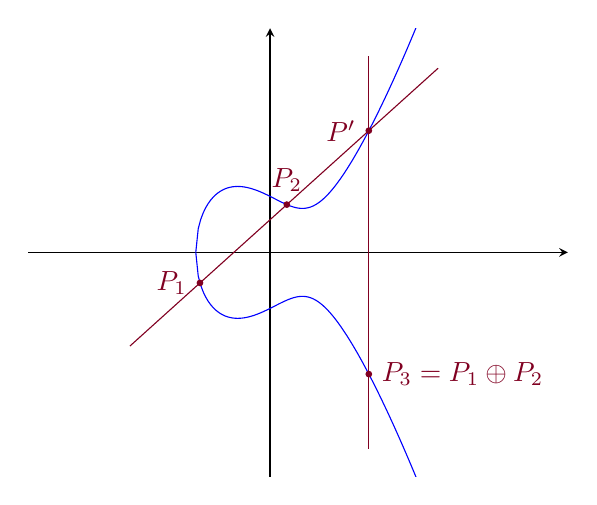
\begin{tikzpicture}
    \begin{axis}[
      xmin = -2, xmax = 3, ymin = -4, ymax = 4,
      axis equal,
      ticks = none,
      axis lines = middle,
      ]
      \addplot[domain=-1.32471796:3, blue, samples=100] {sqrt(x^3-x+1)};
      \addplot[domain=-1.32471796:3, blue, samples=100] {-sqrt(x^3-x+1)};
      \node[circle, burgundy, draw, fill, inner sep=0pt, minimum size=2pt, label={left:\textcolor{burgundy}{$P_1$}}] (P1) at (axis cs:-1.25,-0.54486) {};
      \node[circle, burgundy, draw, fill, inner sep=0pt, minimum size=2pt, label={above:\textcolor{burgundy}{$P_2$}}] (P2) at (axis cs:0.3,0.85264) {};
      \node[circle, burgundy, draw, fill, inner sep=0pt, minimum size=2pt, label={left:\textcolor{burgundy}{$P'$}}] (P3) at (axis cs:1.763, 2.17180) {};
      \addplot[domain=-2.5:3, burgundy] {0.90161*x+0.58216};
      \addplot[burgundy, mark=none] coordinates {(1.763, -3.5) (1.763, 3.5)};
      \node[circle, burgundy, draw, fill, inner sep=0pt, minimum size=2pt, label={right:\textcolor{burgundy}{$P_3 = P_1 \oplus P_2$}}] (P4) at (axis cs:1.763, -2.17180) {};
    \end{axis}
  \end{tikzpicture}
\end{figure}
and put $P_i = (x_i, y_i)$, $P'=(x',y')$.

Now $\ominus P_1 = (x_1, -(a_1x_1+a_3)-y_1)$, just by setting $y = -y_1$ in $(\ast)$.

The line through $P_1, P_2$ has equation say $y = \lambda x + \nu$. Substituting into $(\ast)$ and looking at the coefficient of $x^2$, we get:
\[\lambda^2 + a_1 \lambda - a_2 = x_1 + x_2 + x'\]
Since $x_3 = x'$, we have:
\begin{align*}
   x_3 &= \lambda^2+a_1\lambda-a_2-x_1-x_2\\
   y_3 &= -(a_1 x' + a_3) - y'\\
   &= -(\lambda+a_1)x_3 - \nu - a_3
\end{align*}
It remains to find $\lambda$ and $\nu$. There are 3 cases:
\begin{enumerate}
  \item $x_1=x_2, P_1 \neq P_2$.

  Then $P_1 \oplus P_2 = O_E$.

  \item $x_1 \neq x_2$.

  \[\lambda = \frac{y_2-y_1}{x_2-x_1},\;\; \nu = y_1-\lambda x_1 = \frac{y_1x_2-y_2x_1}{x_2-x_1}\]

  \item $P_1 = P_2$.

  Here we have to compute the equation of the tangent line etc. The solutions are:
  \[ \lambda=\frac{3x_1^2+2a_2x_1+a_4-a_1y_1}{2y_1+a_1x_1+a_3},\;\;\nu = \frac{-x_1^3+a_4x_1+2a_6-a_3y_1}{2y_1+a_1x_1+a_3}\]
\end{enumerate}

\begin{corollary}
  $E(K)$ is an abelian group.
\end{corollary}
\begin{proof}
  It is a subgroup of $E$ ($=E(\bar{K})$).

  \begin{itemize}[leftmargin=2cm]
    \item[Identity:] $O_E \in E(K)$ by definition.
    \item[Closure:] See formulae above.
    \item[Inverses:] See formulae above.
    \item[Associativity:] Inherited from $E(\bar{K})$.
    \item[Commutativity:] Inherited from $E(\bar{K})$.
  \end{itemize}
\end{proof}

If there is no ambiguity (i.e. we are not also adding numbers at the same time), the circles will be dropped from the group operation.
\begin{theorem}
  Elliptic curves are group varieties.

  i.e., $[-1]:E \to E; P\mapsto -P$ and $+:E\times E \to E; (P,Q)\mapsto P+Q$ are morphisms of algebraic varieties.
\end{theorem}
\begin{proof}
  The above formulae show that $[-1]$ and $+$ are rational maps. We know immediately that $[-1]$ is a morphism, as it is a rational map from a smooth curve to a projective variety.

  The formulae also show that $+$ is regular on the set
  \[ U = \{(P,Q) \in E \times E \mid P, Q, P+Q, P-Q \neq O_E\}\]
  For $P \in E$, let $\tau_P:E \to E; X \mapsto P+X$ be the ``translation by $P$" map.

  Then $\tau_P$ is a rational map from a smooth curve to a projective variety, so is a morphism.

  We factor $+$ as:
  \[ E\times E\xrightarrow[\tau_{-A}\times \tau_{-B}]{}E\times E \xrightarrow[\tau_{A+B}]{} E \xrightarrow[\tau_{A+B}]{} E\]

  Now $+$ is regular on $(\tau_A \times \tau_B)(U)$ for all $A, B \in E$, and so $+$ is regular on $E \times E$.
\end{proof}

\underline{\textbf{Definition.}} For any $n \in \Z_{>0}$, let $[n]: E \to E; P \mapsto P+\ldots+P$, $n$ times, and $[-n] = [-1]\circ [n]$, $[0]:P \mapsto O_E$ (i.e., the standard way of turning an abelian group into $\Z$ module).

\underline{\textbf{Definition.}} The \emph{n-torsion} subgroup of $E$ is $E[n] = \ker([n]:E\to E)$.

\begin{lemma}
  If $\charr(K) \neq 2$, and $E : y^2 = (x-e_1)(x-e_2)(x-e_3)$.

  Then $E[2] = (0, (e_1, 0), (e_2, 0), (e_3 0)) \cong (\Z/2\Z)^2$.
\end{lemma}
\begin{proof}
  Let $P = (x, y) \in E$. Then $[2]P = 0 \iff P = -P \iff (x, y) = (x, -y) \iff y = 0$.
\end{proof}

\subsection{Elliptic Curves over $\C$}
Let $\Lambda = \{a\omega_1 + b\omega_2 : a, b \in \Z\}$, where $\omega_1, \omega_2$ form a basis for $\C$ over $\R$.

Then the meromorphic functions on the Riemann surface (or lattice) $\C/\Lambda$ are the same as the $\Lambda$-invariant meromorphic functions on $\C$ (i.e. $f(z) = f(z+\lambda)$ for $\lambda \in \Lambda$).

This set of functions is a field, and is generated by $\wp(z)$ and $\wp'(z)$, where:
\begin{align*}
  \wp(z) = \frac{1}{z^2} + \sum_{0 \neq \lambda\in\Lambda} \left(\frac{1}{(z-\lambda)^2} - \frac{1}{\lambda^2}\right)
\end{align*}
They satisfy $\wp'(z)^2 = 4\wp(z)^3-g_2\wp(z)-g_3$, for some $g_1, g_3 \in \C$ depending on $\lambda$. We call $\wp$ the \emph{Weierstrass p-function}.

One can show that $\C/\Lambda \cong E(\C)$, where $E$ is the elliptic curve $y^2=4x^3-g_2x-g_3$. This is an isomorphism, not only of Riemann surfaces, but moreover of groups

\begin{theorem}[Uniformisation Theorem]
  Every elliptic curve over $\C$ arises in this way.
\end{theorem}

Thus, for elliptic curves $E/\C$, we have:
\begin{enumerate}[label=\protect\circled{\arabic*}]
  \item $E[n] \cong (\Z/n\Z)^2$
  \item $\deg[n] = n^2$
\end{enumerate}
We will show that \circled{2} holds over any field $K$, and \circled{1} holds if $\charr K \nmid n$.

\underline{Summary of Results} (N.B. the isomorphisms in 1, 2, 4 respect the relevant topologies)
\begin{enumerate}
  \item $K = \C$\hspace{2cm}$E(\C) \cong \C/\Lambda \cong \R/\Z\times \R/\Z$
  \item $K = \R$\hspace{2cm}$E(\R) \cong \begin{cases} \Z/2\Z \times \R/\Z & \Delta > 0 \\ \R/\Z & \Delta < 0\end{cases}$
  \item $K = \F_q$\hspace{1.9cm}$|\#E(\F_q) - (q+1)|\leq 2\sqrt{q}$
  \item $[K:\Q_p]<\infty$\hspace{1cm}$E(K)$ has a subgroup of finite index isomorphic to $(\O_K, +)$
  \item $[K:\Q]<\infty$\hspace{1.15cm}$E(K)$ is a finitely generated abelian group.
\end{enumerate}

\section{Isogenies}
Let $E_1, E_2$ be elliptic curves.

\textbf{Definition.} An \emph{isogeny} $\phi:E_1 \to E_2$ is a non-constant morphism taking $O_{E_1}$ to $O_{E_2}$, and we say $E_1$ and $E_2$ are \emph{isogenous} if there is an isogeny $E_1 \to E_2$.

\textbf{Definition.} $\Hom(E_1, E_2) = \{\text{isogenies } E_1 \to E_2\}\cup\{0\}$. This is a group under $(\phi+\psi)(P) = \phi(P)+\psi(P)$.

If $E_1 \xrightarrow{\phi} E_2 \xrightarrow{\psi} E_3$ are isogenies, then $\psi\phi$ is an isogeny. The tower law tells us that $\deg(\psi\phi) = \deg(\phi)\deg(\psi)$.

\begin{lemma}
  If $0 \neq n \in \Z$, then $[n] : E \to E$ is an isogeny.
\end{lemma}
\begin{proof}
  Theorem \textbf{4.4} tells us that $[n]$ is a morphism. We must show that $[n]\neq 0$.

  Assume $\charr K \neq 2$, then we can use Lemma \textbf{4.5}. If $n=2$, then $\#E[2] = 4$, and so $[2] \neq 0$.

  If $n$ is odd, then there is $0\neq T \in E[2]$. Then $nT = T \neq 0$, so $[n]$ is not the zero map.

  Now $[m][n] = [m]\circ[n]$, and any $n = 2^k m$ for $m$ odd, so $[n]$ is not the zero map for any $n \neq 0$.

  If $\charr K =2$, then replace \textbf{4.5} with a lemma computing $E[3]$.
\end{proof}
\textbf{Corollary.} \textit{$\Hom(E_1, E_2)$ is torsion-free as a $\Z$-module.}
\begin{lemma}
  Let $\phi:E_1 \to E_2$ be an isogeny. Then $\phi(P+Q) = \phi(P) + \phi(Q)$ for all $P, Q \in E_1$.
\end{lemma}
\begin{proof}[Sketch proof.]
  $\phi$ induces a map $\phi_\ast : \Div^0(E_1) \to \Div^0(E_2)$ given by $\sum\limits_{P\in E_1}n_p P \mapsto \sum\limits_{P \in E_1}n_p \phi(P)$.

  Recall that, via a pullback, $\phi^\ast : K(E_2) \injection K(E_1)$.

  If $f \in K(E_1)^\ast$, then $\phi_\ast(\div f)=\div(N_{K(E_1)/K(E_2)}f)$ - this is a fact that we'll take for granted.

  So $\phi_\ast$ takes principal divisors to principal divisors. Since $\phi(O_{E_1}) = O_{E_2}$, the following diagram commutes:
  \begin{tikzcd}
    E_1 \arrow{r}{\phi} \arrow{d}{\psi_1} & E_2 \arrow{d}{\psi_2}\\
    \Pic^0(E_1) \arrow{r}{\phi_\ast} & \Pic^0(E_2)
  \end{tikzcd}
  ,where $\psi_1:P \mapsto [(P) -(O_{E_1})], \psi_2:Q \mapsto [(Q)-(O_{E_2})]$.

  Since $\phi_\ast$ is a group homomorphism, $\phi$ is also a group homomorphism.
\end{proof}

\begin{lemma}
  Let $\phi:E_1\to E_2$ be an isogeny. Then there is a morphism $\xi$ making the following diagram commute:

  \begin{center}
    \begin{tikzcd}
      E_1 \arrow{r}{\phi} \arrow{d}{x_1} & E_2 \arrow{d}{x_2} \\
      \P^1 \arrow{r}{\xi} & \P^1
    \end{tikzcd}
  \end{center}

  where $x_i$ is the $x$-coordinate in a Weierstrass equation for $E_i$.

  Moreover, if $\xi(t) = \frac{r(t)}{s(t)}$ for $r, s \in K[t]$ coprime, then $\deg \phi = \deg \xi = \max(\deg r, \deg s)$.
\end{lemma}
\begin{proof}
  For $i = 1,2$, $K(E_i)/K(x_i)$ is a degree 2 extension, since the extension is given by adjoining $y_i$, which satisfies a quadratic (see the Weierstrass equation). Moreover, it is Galois, as $[-1]^\ast$ is a non-trivial automorphism of $K(E_i)$ fixing $K(x_i)$.

  Since $\phi$ is a group homomorphism, we have that $\phi(-P) = -\phi(P)$, i.e. $\phi \circ [-1] = [-1]\circ \phi$.

  If $f \in K(x_2)$, then $[-1]^\ast f = f$, and $[-1]^\ast (\phi^\ast f) = \phi^\ast ([-1]^\ast f) = \phi^\ast f$. Hence $\phi^\ast f$ is fixed by $[-1]$, so is in $K(x_1)$, and $K(x_2) \leq K(x_1)$.

  Taking $f = x_2$, then $\phi^\ast x_2 \in K(x_1)$, say $\xi(x_1)$ for some rational function $\xi$. Then $\xi$ is as required.

  Since $[K(E_1):K(x_1)] = [K(E_2):K(x_2)] = 2$, we have the following diagram of field extensions:
  \begin{center}
    \begin{tikzcd}
      & K(E_1) \arrow[dash, swap]{dl}{2} \arrow[dash]{dr}{\deg\phi} & \\
      K(x_1) \arrow[dash, swap]{dr}{\deg\xi} & & K(x_2) \arrow[dash]{dl}{2}\\
      & K(x_2) &
    \end{tikzcd}
  \end{center}
  Using the tower law, $\deg \phi = \deg \xi$. Now, $K(x_2) \injection K(x_1)$ via $x_2 \mapsto \xi(x_1) = \frac{r(x_1)}{s(x_2)}$ for $r, s \in K[t]$ coprime.

  The minimal polynomial of $x_1$ over $K(x_2)$ is $f(t) = r(t)-s(t)x_2 \in K(x_2)[t]$ - this is clearly a polynomial for $x_1$, but we need to check it's irreducible.

  $f$ is irreducible in $K[t][x_2] = K[x_2][t]$ as it is of degree 1 in $x_2$, so one of the factors must be constant in $x_2$, so divide both $r$ and $s$ which are coprime. Then we can use Gauss's lemma, and it is irreducible in $K(x_2)[t]$.

  Hence $\deg \phi = \deg \xi = [K(x_1):K(x_2)] = \deg (r(t)-s(t)x_2) = \max(\deg r, \deg s)$.
\end{proof}

\begin{lemma}
  $\deg[2] = 4$
\end{lemma}
\begin{proof}
  Assume $\charr K \neq 2, 3$. Then $E: y^2=x^3+ax+b=f(x)$.

  If $P = (x,y)$, then $x(2P) = \left(\frac{3x^2+a}{2y}\right)^2-2x = \frac{(3x^2+a)^2-8xf(x)}{4f(x)} = \frac{x^4+\ldots}{4f(x)}$.

  The numerator and denominator are coprime - suppose there was a common factor. Then $\exists \theta \in \bar{K}$ with $f(\theta) = (3\theta^2+a)^2 = f'(\theta) = 0$, and so $f$ has a multiple root. But $E$ is an elliptic curve so $f$ doesn't have multiple roots.

  Hence $\deg [2] = \max(\deg x^4+\ldots, \deg 4f(x)) = \max(4, 3) = 4$.
\end{proof}

\textbf{Definition.} Let $A$ be an abelian group. We say that $q:A \to \Z$ is a \emph{quadratic form} if it satisfies
\begin{enumerate}
  \item $q(nx) = n^2q(x) \forall n \in \Z, x \in A$.
  \item $(x,y) \to q(x+y)-q(x)-q(y)$ is $\Z$-bilinear.
\end{enumerate}
\begin{lemma}
  $q:A \to \Z$ is a quadratic form if and only if it satisfies the parallelogram law:
  \[q(x+y)+q(x-y) = 2q(x)+2q(y) \forall x,y \in A\]
\end{lemma}
\begin{proof}
  For the forwards direction, let $\angle{x,y} = q(x+y)-q(x)-q(y)$.

  Then $\angle{x,x} = q(2x)-2q(x) = 2q(x)$.

  Then $\frac{1}{2}\angle{x+y,x+y} + \frac{1}{2}\angle{x-y,x-y} = \angle{x,x}+\angle{y,y}$ by bilinearity, and hence $q(x+y)+q(x-y) = 2q(x)+2q(y)$.

  The reverse direction is left as an exercise on example sheet 2.
\end{proof}
\begin{theorem}
  \[\deg : \Hom(E_1, E_2) \to \Z\]
  is a quadratic form.
\end{theorem}
\begin{proof}
For the proof, we will assume $\charr K \neq 2, 3$ for simplicity - the result still holds in those characteristics.

We write $E_2: y^2=x^3+ax+b$.

Let $P, Q \in E_2$ with $P, Q, P+Q, P-Q \neq 0$, and let $x_1, \ldots, x_4$ be the $x$-coordinates of these 4 points. Then we have:
\begin{lemma}
  There exists $w_0, w_1, w_2 \in \Z[a,b][x_1,x_2]$ of degree $\leq 2$ in $x_1$ and in $x_2$ such that $(1:x_3+x_4:x_3x_4) = (w_0:w_1:w_2)$.
\end{lemma}
\begin{proof}
  We could prove this by direct calculation, leading to the formulae:
  \begin{align*}
    w_0 &= (x_1-x_2)^2\\
    w_1 &= 2(x_1x_2+a)(x_1+x_2)+4b\\
    w_2 &= x_1^2x_2^2-2ax_1x_2-4b(x_1+x_2)+a^2
  \end{align*}

  As an alternative proof, let $y=\lambda x +\nu$ be the line through $P$ and $Q$. Then
  \[x^3+ax+b-(\lambda x+\nu)^2 = (x-x_1)(x-x_2)(x-x_3) = x^3-s_1x^2+s_2x-s_3\]
  where $s_i$ is the $i\th$ symmetric polynomial in $(x_1, x_2, x_3)$.

  Comparing coefficients:
  \begin{align*}
    \lambda^2 &= s_1\\
    -2\lambda\nu+a &= s_2\\
    \nu^2-b &=  s_3
  \end{align*}
  Eliminating $\lambda, \nu$, we have $F(x_1, x_2, x_3) \coloneqq (s_2-a)^2-4s_1(s_3+b)=0$. Then $F$ has degree at most 2 in each $x_i$.

  $x_3$ is a root of the quadratic polynomial $W(t) = F(x_1, x_2, t)$, and repeating this for the line through $P$ and $-Q$ shows that $x_4$ is the other root. Hence
  \[w_0(t-x_3)(t-x_4) = W(t) = w_0t^2-w_1t+w_2\]
  And so $(1:x_3+x_4:x_3x_4) = (w_0:w_1:w_2)$.
\end{proof}

We then show that, if $\phi, \psi \in \Hom(E_1, E_2)$, then
\[ \deg(\phi+\psi) +\deg(\phi-\psi) \leq 2\deg(\phi)+2\deg(\psi)\]
We may assume $\phi, \psi, \phi+\psi, \phi-\psi != 0$, as otherwise the result is trivial.

\begin{align*}
  \phi&: (x, y) \mapsto (\xi_1(x), \ldots)\\
  \psi&: (x, y) \mapsto (\xi_2(x), \ldots)\\
  \phi+\psi&: (x, y) \mapsto (\xi_3(x), \ldots)\\
  \phi-\psi&: (x, y) \mapsto (\xi_4(x), \ldots)
\end{align*}
Then \textbf{5.7} gives $(1:\xi_3+\xi_4:\xi_3\xi_4) = ((\xi_1-\xi_2)^2:\ldots:\ldots)$.

Put $\xi_i = \frac{r_i}{s_i}$ where $r_i, s_i \in K[x]$ are coprime:
\[(s_3 s_4:r_3 s_4+r_4 s_3:r_3 r_4) = ((r_1 s_2-r_2 s_2)^2:\ldots:\ldots)\tag{$\ast$}\]

So we have:
\begin{align*}
  \deg(\phi+\psi)+\deg(\phi-\psi) &= \max(\deg r_3, \deg s_3)+\max(\deg r_4, \deg s_4) \\
  &= \max(\deg(s_3s_4), \deg(r_3s_4+r_4s_3), \deg(r_3r_4))
\end{align*}
Suppose $(s_3s_4, r_3s_4+r_4s_3, r_3r_4)$ are not coprime, so that $p$ irreducible divides all $3$. Then $p$ divides one of $r_3, r_4$, and one of $s_3, s_4$. $p$ can't divide both $s_i$ and $r_i$ as they are coprime, so \textsc{wlog} $p$ divides $r_3$ and $s_4$ and not $r_4$ nor $s_3$. Then $p$ doesn't divide $r_3s_4+r_4s_3 \contr$. Hence these polynomials are coprime.

Hence the polynomials on \textsc{rhs} of $(\ast)$ must be multiples of polynomials on the \textsc{lhs} by some irreducible polynomial, and hence each have degree $\geq$ their corresponding polynomial on \textsc{lhs}, and thus, as $w_i$ are of degree $\leq 2$ in $r_1, s_1, r_2, s_2$,
\begin{align*}
  \deg(\phi+\psi)+\deg(\phi-\psi) &\leq \max(\deg(w_0), \deg(w_1), \deg(w_2))\\
  &\leq 2\max(\deg r_1, \deg s_1) + 2\max(\deg r_2, \deg s_2)\\
  &= 2 \deg \phi + 2 \deg \psi\tag{1}
\end{align*}
Now replace $\phi$ and $\psi$ by $\phi+\psi$ and $\phi-\psi$ to get
\[\deg(2\phi)+\deg(2\psi) \leq 2\deg(\phi+\psi)+2\deg(\phi-\psi)\]
Since $\deg[2] = 4$,
\[2\deg(\phi)+2\deg(\psi) \leq \deg(\phi+\psi)+\deg(\phi-\psi)\tag{2}\]
(1) and (2) together give
\[ 2\deg(\phi)+2\deg(\psi) = \deg(\phi+\psi)+\deg(\phi-\psi)\]
so $\deg$ satisfies the parallelogram law, and hence is a quadratic form.
\end{proof}
\begin{corollary}
  \[deg(n\phi) = n^2\deg(\phi) \forall n\in \Z, \phi \in \Hom(E_1, E_2)\]
  In particular, $\deg[n] = n^2$.
\end{corollary}
\stepcounter{theorem}
\textbf{Example \thetheorem.} Let $E/K$ be an elliptic curve, suppose $\charr K \neq 2$, and let $O_E \neq T \in E(K)[2]$.

Then we may take $E: y^2 = x(x^2+ax+b), a, b \in K, b(a^2-4b) \neq 0$, $T=(0, 0)$

Then if $P=(x,y)$ and $P'=P+T = (x', y')$, then:
\begin{align*}
  x' &= (y/x)^2 - a - x = \frac{x^2+ax+b}{x}-x-a- = \frac{b}{x}\\
  y' &= -(y/x)x' = \frac{-by}{x^2}
\end{align*}
Then let $\xi = x+x'+a = \frac{x^2+ax+b}{x} = \left(\frac{y}{x}\right)^2$, and $\eta = y+y' = \frac{y}{x}(x-\frac{b}{x})$

Then $\eta^2=\left(\frac{y}{x}\right)^2\left[\left(x+\frac{b}{x}\right)^2-4b\right] = \xi\left((\xi-a)^2-4b\right) = \xi(\xi^2-2a\xi+a^2-4b)$

Let $E': y^2=x(x^2+a'x+b')$ where $a' = -2a, b'=a^2-4b$. Then there is an isogeny $\phi:E \to E'$ given by $(x, y) \mapsto \left(\left(\frac{y}{x}\right)^2:\frac{y(x^2-b)}{x^2}:1\right); O_E \mapsto (0:1:0)$

\textbf{5.3} tells us, as $x' = \left(\frac{y}{x}\right)^2 = \frac{x^2+ax+b}{x}$, that $\deg(\phi) = \max(2,1) = 2$, and we say $\phi$ is a 2-isogeny.

\section{The Invariant Differential}
Let $C$ be an algebraic curve over an algebraically closed field. Then the \emph{space of differentials} $\Omega_C$ is a vector space over the function field of the curve $K(C)$, generated by $df$ for $f \in K(C)$ subject to the relations
\begin{enumerate}
  \item $d(f+g) = df+dg$
  \item $d(fg) = fdg+gdf$
  \item $da = 0$ for $a \in K$
\end{enumerate}
It turns out that $\dim \Omega_C = \dim C$, and since $C$ is a curve, $\Omega_C$ is a 1-dimensional $K(C)$-vector space.

Let $0\neq \omega \in \Omega_C$, and let $P \in C$ be a smooth point, with $t \in K(C)$ a uniformizer at $P$ (has order of vanishing 1 at $P$). Then $\omega = fdt$ for some $f \in K(C)$.

We define $\ord_P(\omega) = \ord_P(f)$. This does not depend on the choice of uniformizer.

Suppose we have $f \in K(C)^\ast$, and $\ord_P(f) = n \neq 0$. Then, if $\charr K \nmid n$, $\ord_P(df) = n-1$.

If $C$ is now a smooth projective curve, we define the divisor of $\omega \in \Omega_C$ to be
\[\div(\omega) = \sum_{P \in C} \ord_P(\omega) P \in \Div(C)\]
using the fact that $\ord_P(\omega)$ is zero at all but finitely many points $P \in C$.

The \emph{space of regular differentials} is the finite dimensional vector space over $K$ of all $\omega \in \Omega_C$ for which $\div(\omega)$ is effective, i.e. there are no poles. The dimension of this space is called the \emph{genus} of $C$, $g(C)$.

As a consequence of Riemann-Roch, we have, for $0 \neq \omega \in \Omega_C$, $\deg(\div(\omega)) = 2g(C)-2$.

\begin{lemma}
  Assume $\charr K \neq 2$. Take an elliptic curve $E:y^2=(x-e_1)(x-e_2)(x-e_3)$, where $e_1, e_2, e_3$ distinct.

  Then $\omega = \frac{dx}{y}$ is a differential on $E$, and has no zeros and no poles, and so $g(E)=1$.

  Moreover, the space of regular differentials is just $\angle{\omega}$.
\end{lemma}
\begin{proof}
  Let $T_i = (e_i, 0)$, so that $E[2] = \{O, T_1, T_2, T_3\}$.

  Then $\div(y) = (T_1)+(T_2)+(T_2)-3(O)$ - we know the zeros at $T_i$ are simple as $y$ is rational, so $\deg \div(y) = 0$.

  Then for $P \in E, \div(x-x_P) = (P) + (-P) - 2(O)$, in the same way as above.

  If $P \in E\setminus E[2]$, then $\ord_P(x-x_P) = 1$, so $\ord_P(d(x-x_P)) = \ord_P(dx) = 1-1= 0$.

  If $P = T_i$, then $P = -P$, and $\ord_P(x-x_p) = 2$, so $\ord_P(dx) = 2-1 = 1$

  If $P = O$, then $\ord_P(x) = -2$, so $\ord_P(dx) = -3$.

  Hence $\div(dx) = (T_1)+(T_2)+(T_3)-3(O) = \div(y)$.

  So $\div(dx/y) = \div(dx)-\div(y) = 0$. Then Riemann-Roch gives $g(E) = 1$, and so the space of regular differentials is 1-dimensional, so generated by $\omega$.
\end{proof}
\textbf{Definition.} If $\phi:C_1 \to C_2$ is a non-constant morphism, then we can pull back to \[\phi^\ast:\Omega_{C_1}\to \Omega_{C_2}; fdg \mapsto \phi^\ast f d(\phi^\ast g)\]

\begin{lemma}
  Let $P \in E$, $\tau_P:E \to E; X \mapsto P+X$, and $\omega = dx/y$ be as above.

  Then $\tau_P^\ast \omega = \omega$, and so $\omega$ is called the \emph{invariant differential}.
\end{lemma}
\begin{proof}
  Since $\omega$ had no poles, $\tau_P^\ast \omega$ is again a regular differential, and hence equal to $\lambda_P \omega$ for some $\lambda_P \in K$, as the regular differentials are a 1-dimensional vector space over $K$.

  The map $E \to \P^1; P \mapsto \lambda_P$ is a morphism of smooth projective curves, but is not surjective as it misses $0$ and $\infty$, and so this morphism is constant, by \textbf{2.8}.

  So $\lambda$ is independent of $P$. Take $P = O_E$, then $\tau_P$ is the identity map, and so $\lambda$ is 1.
\end{proof}
If $K = \C$, then $\C/\Lambda \cong E(\C)$, via $z \mapsto (\wp(z), \wp'(z))$. Then $\frac{dx}{y}=\frac{\wp'(z)dz}{\wp'(z)} = dz$, which is invariant under $z \mapsto z+\text{const.}$.

\begin{lemma}
  Let $\phi, \psi \in \Hom(E_1, E_2)$, $\omega$ the invariant differential on $E_2$. Then \[(\phi+\psi)^{\ast}(\omega) = \phi^{\ast}\omega + \psi^{\ast}\omega\]
\end{lemma}
\begin{proof}
  Write $E=E_2$, and consider the maps:
  \begin{align*}
    E\times E &\to E\\
    \upmu:(P, Q) &\mapsto P+Q\\
    \text{pr}_1:(P,Q) &\mapsto P\\
    \text{pr}_2:(P,Q) &\mapsto Q
  \end{align*}
  $\Omega_{E\times E}$ is a 2-dimensional $K(E\times E)$ vector space with basis $\text{pr}_1^\ast \omega$ and $\text{pr}_2^\ast \omega$.

  Then $\upmu^\ast \omega = f \text{pr}_1^\ast \omega + g\text{pr}_2^\ast \omega$ for some $f, g \in K(E\times E)$.

  For $Q \in E$, let $\iota_Q : E \to E\times E; P \mapsto (P, Q)$. Then

  \begin{align*}
    \iota_Q^\ast(\upmu^\ast \omega) = (\upmu\circ\iota_Q)^\ast \omega &= \iota_Q^\ast f(\text{pr}_1\circ \iota_Q)^\ast\omega + \iota_Q^\ast g (\text{pr}_2\circ \iota_Q)^\ast \omega\\
    \tau_Q^\ast \omega &= \iota_Q^\ast f \omega + 0\\
    \omega &= \iota_Q^\ast f \omega
  \end{align*}
  So $\iota_Q^\ast f = 1$ for all $Q \in E$, so $f(P,Q) = 1$ for all $P, Q \in E$.

  Similarly, $g(P,Q) = 1$.

  So $\mu^{\ast} \omega= \text{pr}_1^\ast \omega + \text{pr}_2^\ast \omega$. Now pull back by $E\to E\times E; P \mapsto (\phi(P), \psi(P))$ to get $(\phi+\psi)^\ast \omega=  \phi^\ast \omega + \psi^\ast \omega$.
\end{proof}
\begin{lemma}
  If $\phi:C_1 \to C_2$ is a non-constant morphism, then $\phi$ is separable if and only if $\phi^\ast:\Omega_{C_2}\to \Omega_{C_1}$ is nonzero
\end{lemma}
\begin{proof}
  Omitted.
\end{proof}
\underline{Example:} Let $\mathbb{G}_m = \A^1\setminus\{0\} = \P^1\setminus\{0, \infty\}$, with group law $\mathbb{G}_m \times \mathbb{G}_m \to \mathbb{G}_m; (x,y)\mapsto xy$.

Let $n \geq 2$ be an integer, $\alpha:\G_m \to \G_m; x\mapsto x^n$.

Then $\alpha^{\ast}(dx) = d(\alpha x) =d(x^n) = nx^{n-1}dx$. So if $\charr K \nmid n$, then $\alpha$ is separable. So $\# \alpha^{-1}(Q) = \deg \alpha$ for all but finitely many $Q \in \mathbb{G}_m$.

But $\alpha$ is group homomorphism, so all fibres have the same size, and $\#\alpha^{-1}(Q) = \#\ker \alpha$, hence $\# \ker \alpha = \deg \alpha=n$. So $K (=\bar{K})$ contains exactly $n$ $n\th$ roots of unity.

\begin{theorem}
  If $\charr K \nmid n$, then $E[n] \cong (\Z/n\Z)^2$.
\end{theorem}
\begin{proof}
  By \textbf{6.3} and induction, $[n]^\ast \omega = n\omega$. So if $\charr K \nmid n$, $[n]$ is separable. So all but finitely many fibres of $[n]$ have size $\deg [n]$, and since $[n]$ is a group homomorphism, all fibres have the same size, and hence $\#[n]^{-1}(O_E) = \#E[n] = \deg [n] = n^2$.

  By the structure theorem for finite abelian groups, $E[n] \cong \Z/d_1\Z \times \ldots \Z/d_t\Z$ with $d_i | d_{i+1}$. Since this group is killed by multiplication by $n$, all $d_i| n$ as well, and $\prod_{i=1}^t d_i = n^2$ by the previous paragraph.

  If $p$ is a prime with $p | d_1$, then $E[p] \cong (\Z/p\Z)^t$, and by the first paragraph, $t=2$. Then $d_1|d_2|n$, and $d_1d_2 = n^2$, hence $d_1=d_2 = n$.
\end{proof}
Remark (not to be used on example sheet 2). If $\charr K = p$, then $[p]$ is not separable. It can be shown that $E[p^r] \cong \Z/p^r\Z$ for all $r \geq 1$ or $E[p] = 0$. The first case is described as ``ordinary", and the second case is ``supersingular".

\section{Elliptic Curves over Finite Fields}
\begin{lemma}
  Let $A$ be an abelian group and $q:A \to \Z$ a positive definite quadratic form. If $x, y \in A$ then $\angle{x, y}\coloneqq |q(x + y)-q(x)-q(y)|\leq 2 \sqrt{q(x)q(y)}$.
\end{lemma}
\begin{proof}
  We may assume $x \neq 0$ otherwise the result is clear. Let $m,n \in \Z$.
  \begin{align*}
      0 & \leq q(mx+ny)\\
      &=\frac{1}{2}\angle{mx+ny,mx+ny} \\
      &= m^2q(x) + mn\angle{x,y} + n^2q(y)\\
      &= q(x)\left(m+\frac{\angle{x,y}}{2q(x)}n\right)^2 + n^2\left(q(y)-\frac{\angle{x,y}^2}{4q(x)}\right)
  \end{align*}
  Take $m = \angle{x,y}, n = -2q(x)$, we deduce $\angle{x,y}^2 \leq 4q(x)q(y)$, so $|angle{x,y}| \leq 2\sqrt{q(x)q(y)}$.
\end{proof}
Recall that $\Gal(\F_{q^r}/\F_q)$ is cyclic of order $r$ generated by the Frobenius map $x \mapsto x^q$.
\begin{theorem}[Hasse]
  Let $E/\F_q$ be an elliptic curve. Then $\abs{\#E(\F_q)-(q+1)}\leq 2\sqrt{q}$
\end{theorem}
\begin{proof}
  Let $E$ have Weierstrass equation with coefficients $a_1, \ldots, a_6 \in \F_q$. Define the Frobenius endomorphism $\phi:E \to E; (x,y) \mapsto (x^q, y^q)$, which is an isogeny of degree $q$.

  Then $E(\F_q) = \{P \in E: \phi(P) = P\} = \ker(1-\phi)$.

  $\phi^{\ast}\omega = \phi^\ast\left(\frac{dx}{y}\right) = \frac{dx^q}{y^q} = \frac{qx^{q-1}dx}{y^q} = 0$, since $q \equiv 0 \mod p.$

  So $(1-\phi)^\ast \omega = 1^\ast \omega - \phi^\ast \omega = \omega - 0 = \omega \neq 0$, so $1-\phi$ is separable.

  Hence the size of all but finitely many fibres is $\deg 1-\phi$, and $1-\phi$ is a group homomorphism, so $\#E[\F_q] = \#\ker(1-\phi) = \deg(1-\phi)$.

  By \textbf{5.6}, $\deg :\text{End}(E) \coloneqq \Hom(E,E) \to \Z$ is a positive definite quadratic form.

  By \textbf{7.1}, $|\deg(1-\phi)-1-\deg\phi| \leq 2\sqrt{\deg \phi}$, and hence $|\#E(\F_q) - (q+1)| \leq 2\sqrt{q}$.
\end{proof}

\subsection{Zeta Functions}
For $K$ a number field:
\[\zeta_K(s) = \sum_{\mathfrak{a} \subset \O_K} \frac{1}{(N_{\mathfrak{a}})^s} = \prod_{\mathfrak{p}\subset \O_K \text{ prime}} \left(1-\frac{1}{(N_{\mathfrak{p}})^s}\right)^{-1}\]
For $K$ a function field, e.g. $K = \F_q(C)$ for $C/\F_q$ a smooth projective curve:
\[\zeta_K(s) = \prod_{x\in |C|}\left(1-\frac{1}{(Nx)^s}\right)^{-1}\]
where $|C|$ is the set of closed points (i.e. orbit of action of $\Gal(\bar{\F}_q/\F_q))$ on $C(\bar{\F}_q)$, and $Nx = q^{\deg x}$, where $\deg x$ is the size of the orbit.

We have that $\zeta_K(s) = F(q^{-s})$ for $F \in Q[[T]]$, where
\begin{align*}
  F(T) &= \prod_{x \in |C|} (1-T^{\deg x})^{-1}\\
  \log F(T) &= \sum_{x \in |C|} \sum_{m=1}^\infty \frac{1}{m}T^{m\deg x}\\
  \frac{d}{dT} \log F(T) &= \sum_{x \in |C|}\sum_{m=1}^\infty \deg x T^{m \deg x}\\
  &= \sum_{n=1}^\infty \left(\sum_{\substack{x \in |C|\\\deg x |n}} \deg x\right)T^n\\
  &= \sum_{n=1}^\infty \# C(\F_{q^n})T^n\\
  \implies F(T) &= \exp\left(\sum_{n=1}^\infty \frac{\#C(\F_{q^n})}{n}T^n\right) \eqqcolon Z_C(T)
\end{align*}

For $\phi, \psi \in \Hom(E_1, E_2)$, we put:
\[\angle{\phi, \psi} = \deg(\phi+\psi) - \deg(\phi) - \deg(\psi)\]
We define the \emph{trace map} $\tr: \End(E) \to \Z$; $\psi \mapsto \angle{\psi, 1}$.

\begin{lemma}
  If $\psi \in \End(E)$ then $\psi^2 - [\tr\psi]\psi + [\deg \psi] = 0$, where $[n]$ means the multiplication by $n$ endomorphism.
\end{lemma}
\begin{proof}
  Example sheet 2.
\end{proof}
\textbf{Definition.} The \emph{zeta function of a variety} $V/\F_q$ is
\[Z_v(T) = \exp\left(\sum_{n=1}^\infty \frac{\#V(\F_{q^n})}{n}T^n\right)\]
\begin{lemma}
  Let $E/\F_q$ be an elliptic curve, with $\#E(\F_q) = q+1-a$. Then
  \[Z_E(T) = \frac{1+aT+qT^2}{(1-T)(1-qT)}\]
\end{lemma}
\begin{proof}
  Let $\phi: E \to E$ be the $q$-power Frobenius map. By the proof of Hasse's theorem,
  \[\#E(\F_q) = \deg(1-\phi) = q+1-\tr(\phi)\]
  Then $\tr(\phi) = a, \deg(\phi) = q$.

  Then lemma \textbf{7.3} gives $\phi^2 - a\phi+q = 0$. Composing with $\phi^n$ for $n\geq 0$ gives
  \begin{align*}
    \phi^{n+2} - a \phi^{n+1}+q\phi^n &= 0\\
    \tr(\phi^{n+2}) - a \tr(\phi^{n+1}) + q \tr(\phi^n) &= 0
  \end{align*}
  This second-order difference equation with initial conditions $\tr(\phi^0) = \tr(1) = 2, \tr(\phi^1) = a$ has solutions
  \[\tr(\phi^n) = \alpha^n + \beta^n\]
  where $\alpha, \beta$ are the roots of $x^2-ax+q=0$.

  Hence $\#E(\F_{q^n}) = \deg(1-\phi^n) = 1+ \deg(\phi^n) - \tr(\phi^n) = 1+q^n-\alpha^n-\beta^n$.

  Substituting, we have:
  \begin{align*}
    Z_E(T) &= \exp\left(\sum_{n=1}^\infty \frac{T^n}{n} + \frac{(qT)^n}{n} - \frac{(\alpha T)^n}{n} - \frac{(\beta T)^n}{n}\right)
  \end{align*}
  Since $-\log(1-x) =  \sum_{n=1}^\infty \frac{x^n}{n}$, this can be simplified to:
  \begin{align*}
    Z_E(T) &= \frac{(1-\alpha T)(1-\beta T)}{(1-T)(1-qT)}\\
    &= \frac{1-aT+qT^2}{(1-T)(1-qT)}
  \end{align*}
\end{proof}
Note that Hasse's theorem gives us $|a| \leq 2\sqrt{q}$, and so the discriminant of $x^2-aT+q$ is negative, and so $\alpha = \bar{\beta}, |\alpha|=|\beta| = \sqrt{q}$.

Let $K = \F_q(E)$. Then $\zeta_K(s) = 0 \implies Z_E(q^{-s}) = 0 \implies q^2 = \alpha$ or $\beta$, and hence $\Re(s) = \frac{1}{2}$.

\section{Formal Groups}
Here, $R$ will be a ring with $I \subset R$ an ideal. The \emph{I-adic topology} on $R$ is the topology with basis $\{r+I^n: r\in R, n\geq 1\}$.

A sequence $(x_n)$ in $R$ is \emph{Cauchy} if, for all $k$ there is some $N$ with $x_m-x_n \in I^k$ for all $m, n \geq k$.

$R$ is \emph{complete} if
\begin{enumerate}
  \item $\bigcap_{n\geq 0} I^n = \{0\}$ and
  \item every Cauchy sequence converges.
\end{enumerate}
Note that, if $x \in I$ then $\frac{1}{1-x} = 1+x+x^2+\ldots$, and the sequence of partial sums is Cauchy, and hence converges. So $1-x \in R^\times$.

For example, we could have:
\begin{itemize}
  \item $R = \Z_p, I = p\Z_p$
  \item $R = \Z[[t]], I = (t)$.
\end{itemize}
\begin{lemma}[Hensel's Lemma]
  Let $R$ be an integral domain, complete with respect to $I$. Let $F \in R[x], s \geq 1$. Suppose $a \in R$ satisfies $F(a) \equiv 0 \mod I^s$, and $F'(a) \in R^\times$.

  Then there is a unique $b \in R$ with $F(b) = 0$ and $b \equiv a \mod I^s$.
\end{lemma}
\begin{proof}
  Let $u \in R^\times$ with $F'(a) \equiv u \mod I$, e.g. $u = f'(a)$.

  Replacing $F(x)$ by $\frac{F(x+a)}{u}$, we may assume $a = 0$ and $F'(0) \equiv 1 \mod I$.

  We put $x_0 = 0, x_{n+1} = x_n-F(x_n)$.

  By induction, $x_n \in I_s$ for all $n$.

  $F(x)-F(y) = (x-y)(F'(0)+xG(x,y) +yH(x,y))$ for some polynomials $G, H \in R[x,y]$.

  Now we claim $x_{n+1} \equiv x_n \mod I^{n+s}$ for all $n \geq 0$.

  This can be proven by induction on $n$: in the case where $n=0$, and $x_1 \in I^s$.

  Suppose $x_{n}\equiv x_{n-1} \mod I^{n+s-1}$. Then
  \[F(x_n)-F(x_{n-1})=(x_n-x_{n-1})(1+c)\]
  for some $c \in I$, and hence
  \[F(x_n) - F(x_{n-1}) \equiv x_n-x_{n-1} \mod I^{n+s}\]
  Rearranging, we have $x_{n+1} \equiv x_n \mod I^{n+s}$, which proves the claim.

  Hence $(x_n)$ is Cauchy, and by completeness converges to some $b \in R$. Taking the limit as $n \to \infty$, we have $b = b-F(b)$, and so $F(b)=0$, with $b \in I^s$.

  For uniqueness, we can use the expression for $F(x)-F(y)$ and the assumption that $R$ is an integral domain.
\end{proof}
For example, take $E: Y^2Z + a_1XYZ+a_3YZ^2 = X^3+a_2X^2Z + a_4 XZ^2 + a_6Z^3$

We pass to the affine piece $Y \neq 0, t = X/Y, w = -Z/Y$: Then
\[E : w = t^3+a_1tw + a_2t^2w + a_3w^2+a_4tw^2+a_6w^3 = f(t,w)\]
We can apply Hensel's lemma with $R = \Z[a_1, \ldots, a_6][[t]]$, $I = (t)$, and $F(x) = x-f(t,x)\in R[x]$. Taking $s = 3, a = 0$, we have:
\[F(0) = -f(t, 0) = -t^3 \equiv 0 \mod I^3\;\;\;\;\;\;\;\;
F'(0) = 1-a_t-a_2t^2  \in R^\times\]
So there is a unique root of $F$, $w(t) \in \Z[a_1, \ldots, a_6][[t]]$ such that $w(t) = f(t,w(t))$ and $w(t) \equiv 0 \mod t^3$.

Following the proof of Hensel's lemma with $u = 1$ gives $w(t) = \lim_{n\to \infty} w_n(t)$ where $w_0(t) = 0, w_{n+1}(t)=f(t, w_n(t))$.

In fact, we may write \mbox{$w(t) = \sum_{n=2}^\infty A_{n-2}t^{n-1}$ with $A_1 = a_1, A_2 = a_1^2+a_2, A_3 = a_1^3+2a_1a_2+a_3, \ldots$}

\begin{lemma}
  Let $R$ be an integral domain, complete with respect to $I \trianglelefteq R$, and let $a_1, \ldots, a_6 \in R, K = \Frac(R)$.

  Then $\hat{E}(I) = \{(t,w) \in E(K): t, w \in I\} = \{(t, w(t))\in E(K): t \in I\}$ is a subgroup of $E(K)$.
\end{lemma}
\begin{proof}
  The two descriptions of $\hat{E}(I)$ agree, since given $t \in I$ we can solve for a unique $w \in I$ such that the pair $(t,w)\in E(K)$.

  Taking $(t, w) = (0, 0)$ shows that $O_E \in \hat{E}(I)$. So it suffices to show that, if $P_1, P_2 \in \hat{E}(I)$, then $-P_1-P_2 \in \hat{E}(I)$.

  If $P_1 = (t_1,w_1), P_2 = (t_2,w_2)$ lie on the straight line $\lambda t + \nu$, then $-P_1-P_2$ is the third point of intersection of this line with $E$.

  Then $\lambda = \frac{w(t_2)-w(t_1)}{t_2-t_1}$ if $t_1 \neq t_2$, and $w'(t_1)$ if $t_1=t_2$.

  $P_1, P_2 \in \hat{E}(I) \implies t_1, t_2 \in I$.

  Thus $\lambda = \sum_{n=2}^\infty A_{n-2}(t_1^n + t_1^{n-1}t_2 + \ldots + t_2^n) \in I$, and $\nu = w_1-\lambda t_1 \in I$.

  Substituting $w = \lambda t + \nu$ into $w = f(t,w)$ gives $\lambda t+\nu = t^3 + a_1t(\lambda t+ \nu) + a_2t^2(\lambda t+\nu) + a_3(\lambda t+ \nu)^2 + a_4 t(\lambda t + \nu)^3 + a_6(\lambda t+\nu)^3$.

  Let $A$ be the coefficient of $t^3$, so $A = 1+a_2\lambda+a_4 \lambda^2 + a_6\lambda^3$.

  Let $B$ be the coefficient of $t^2$, so $B = a_1\lambda + a_2\nu + a_3\lambda^2+2a_4\lambda\nu+3a_6\lambda^2\nu$.

  Then $A \in R^\times, B \in I$, and $t_3 = -B/A -t_2 -t_2 \in I$, and $w_3 = \lambda t_3 + \nu \in I$.

  Hence $-P_1-P_2 \in \hat{E}(I)$, and so $\hat{E}(I)$ is a subgroup.
\end{proof}
Taking $R = \Z[a_1, \ldots, a_6][[t]]$, and $I = (t)$, then the previous lemma tells us there is some power series $\iota \in \Z[a_1,\ldots, a_6][[t]]$ with $\iota(0) = 0$ such that $[-1](t, w(t)) = (\iota(t), w(\iota(t)))$

Taking $R = \Z[a_1, \ldots, a_6][[t]]$, and $I=(t_1, t_2)$, then we get that there is some power series $F \in I$ such that $(t_1,w(t_1))+(t_2,w(t_2)) = (F(t_1,t_2),w(F(t_1,t_2))$.

In fact, we can compute
\begin{align*}
  \iota(x) &= -x-a_1x^2-a_2x^3-(a_1^3+a_3)x^4+\ldots\\
  F(x, y) &= x+y-a_1xy-a_2(x^2y+xy^2)+\ldots
\end{align*}
By properties of the group law, we can deduce:
\begin{enumerate}
  \item $F(x, y) = F(y, x)$
  \item $F(x, 0) = x, F(0, y) = y$
  \item $F(x, F(y, z)) = F(F(x, y), z)$
  \item $F(x, \iota(x)) = 0$
\end{enumerate}
This then motivates the following definition:

\textbf{Definition.} Let $R$ be a ring. A \emph{formal group} over $R$ is a power series $F(x, y) \in R[[x, y]]$ satisfying the properties 1, 2, and 3 above.

\textbf{Exercise.} Show that, for any formal group, there is a unique $\iota(x) \in R[[x]]$ such that \mbox{$F(x,\iota(x)) = 0$}.

\underline{Examples:}
\begin{enumerate}
  \item $F(x, y) = x + y$
  \item $F(x, y) = x + y + x y = (1 + x)(1 + y) - 1$
  \item $F$ as above.
\end{enumerate}
We label these formal groups by $\hat{\G}_a, \hat{\G}_m$, and $\hat{E}$ respectively.

\textbf{Definition.} Let $\mathcal{F}$, $\mathcal{G}$ be formal groups over $R$ given by power series $F, G$ respectively. Then:
\begin{enumerate}
  \item A \emph{morphism} $f: \mathcal{F} \to \mathcal{G}$ is a power series $f \in R[[t]]$ such that $f(0)=0$ satisfying $f(F(x, y)) = G(f(x), f(y))$.
  \item $\mathcal{F} \cong \mathcal{G}$ if there is some morphism $f : \mathcal{F} \to \mathcal{G}$, and $g: \mathcal{G} \to \mathcal{F}$ with $f(g(x))=g(f(x)) = x$.
\end{enumerate}
\begin{theorem}
  If $\charr(R) = 0$, then any formal group $\mathcal{F}$ over $R$ is isomorphic to $\hat{\G}_a$ over $R \otimes \Q$.

  More precisely:
  \begin{enumerate}
    \item There is a unique power series $\log: T\mapsto T+\frac{a_2}{2}T^2+\frac{a_3}{3}T^3+\ldots$ with $a_i \in R$, such that \[\log(F(x,y)) = \log(x)+\log(y)\tag{$\ast$}\]
    \item There is a unique power series $\exp: T \mapsto T + \frac{b_2}{2!}T^2 + \frac{b_3}{3!}T^3+\ldots$ with $b_i \in R$ such that \[\exp(\log(T)) = \log(\exp(T)) = T\]
  \end{enumerate}
\end{theorem}
\begin{proof}\hspace*{0cm}
  \begin{enumerate}
    \item Notation: $F_1(x, y) = \frac{\partial F}{\partial x}(x, y)$ (via formal differentiation).

    For uniqueness, let $p(T) = \frac{d}{dT} \log(T) = 1 + a_2T + a_3T^2 + \ldots$.

    Differentiating ($\ast$) with respect to $x$, we get: $p(F(x, y))F_1(x, y) = p(x)+0$
    Setting $x = 0$, we get $p(y)F_1(0, y) = 1$, and hence $p(y) = F_1(0, y)^{-1}$, and hence $p$ is uniquely determined, so $a_2, a_3, \ldots$ are uniquely determined. But then $\log$ is uniquely determined.

    For existence, let $p(T) = F_1(0, T)^{-1} = 1 + a_2T + a_3 T^2 + \ldots$, where $a_i \in R$.

    Integrating up, we let $\log(T) = T + \frac{a_2}{2}T^2+\frac{a_3}{3}T^3+\ldots$. We now check it satisfied ($\ast$).
    \begin{align*}
      F(F(x, y), z) &= F(x, F(y, z))\\
      \frac{\partial}{\partial x} F(F(x,y), z) &= \frac{\partial}{\partial x} F(x, F(y, z))\\
      F_1(F(x, y), z) F_1(x,y) &= F_1(x, F(y, z))\\
      F_1(F(0, y), z) F_1(0,y) &= F_1(0, F(y, z))\\
      F_1(y, z) F_1(0, y) &= F_1(0, F(y, z))\\
      F_1(y,z) p(y)^{-1} &= p(F(y, z))^{-1}\\
      F_1(y, z) p(F(y,z)) &= p(y)\\
      \log(F(y, z)) &= \log(y) + h(z)
    \end{align*}
    By symmetry between $y, z$ we see that the constant of integration $h(z)$ must be $\log (z)$.
  \end{enumerate}
  For the second part, we will need the following lemma, which is a generalisation of the statement:
  \begin{lemma}
    Let $f(T) = aT + \ldots \in R[[T]]$ with $a \in R^\times$. Then there is a unique $g(T) = a^{-1}T+  \ldots \in R[[t]]$ such that $f(g(T)) = g(f(T)) = T$.
  \end{lemma}
  \begin{proof}
    We construct polynomials $g_n(T) \in R[T]$ such that $f(g_n(T)) \equiv T \mod T^{n+1}$ and $g_{n+1}(T) \equiv g_n(T) \mod T^{n+1}$. Then we will set $g(T) = \lim_{n\to\infty} g_n(T)$, satisfying $f(g(T)) = T$.

    This is done inductively. To start with, $g_1(T) = a^{-1}T$. Then $f(g_1(T)) = T+T^2(\ldots) \equiv T \mod T^2$.

    Now suppose $n\geq 1$ and $g_{n-1}(T)$ exists.

    Then $f(g_{n-1}(T)) \equiv T + bT^n \mod T^{n+1}$. Let $g_n(T) = g_{n-1}(T) + \lambda T^n$, where $\lambda \in R$ to be chosen later.

    Then $f(g_n(T)) = f(g_{n-1}(T)+\lambda T^n) \equiv f(g_{n-1}(T)) + \lambda aT^{n} \mod T^{n+1} \equiv T + (b+\lambda a)T^{n} \mod T^{n+1}$.

    So pick $\lambda = -ba^{-1}$.

    This gives $g(T)$ with $f(g(T)) = T$.

    Applying the same argument, we get $h(T)$ such that $g(h(T)) = T$.

    Then $f(T) = f(g(h(T))) = h(T)$, and so $g$ is as required.
  \end{proof}
  \begin{enumerate}
    \item[2.] We now only have to show that the $b_n \in R$ (not just in $R \otimes \Q$). See example sheet 2 for this.
  \end{enumerate}
\end{proof}
Let $\mathscr{F}$ be a formal group (e.g. $\hat{\G}_a, \hat{\G}_m, \hat{E}$), given by a power series $F \in R[x,y]$, and suppose that $R$ is $I$-adically complete. Then for $x, y \in I$, put $x \oplus_{\mathscr{F}} y = F(x,y) \in I$. Then $\mathscr{F} = (I, \oplus_{\mathscr{F}})$ is an abelian group.

For example, $\hat{\G}_a(I) = (I, +), \hat{\G}_m(I) = (1+I, \times)$, and in \textbf{8.2}, we saw $\hat{E}(I) \leq E(K)$.

\begin{corollary}
  Let $\mathscr{F}$ be a formal group over $R$, and $n \in \Z$. Suppose $n \in R^\times$. Then:
  \begin{enumerate}
    \item $[n]:\mathscr{F} \to \mathscr{F}$ is an isomorphism.
    \item If $R$ is complete with respect to $I$, then $\mathscr{F}(I) \xrightarrow{\times n} \mathscr{F}(I)$ is an isomorphism.
  \end{enumerate}
  In particular, $\mathscr{F}(I)$ has no $n$-torsion.
\end{corollary}
\begin{proof}
  We have $[1](T) = T, [n](T) = F([n-1]T, T)$ for $n \geq 2$. For $n < 0$, use $[-1](T) = \iota(T)$.

  Induction gives us $[n](T) = nT + \ldots$, and so by \textbf{8.4}, $[n]$ is an isomorphism.
\end{proof}
\section{Elliptic Curves over Local Fields}
Let $K$ be a field, complete with respect to the discrete valuation $v: K^\times \to \Z$. Then we define the valuation ring, or ring of integers, the set:
\[\O_K = \{x \in K^\times : v(x) \geq 0 \} \cup\{0\}\]
Then $\O_K^\times = \{x \in K^\times : v(x) = 0\}$. There is a unique maximal ideal $\pi \O_K$, where $v(\pi) = 1$, and we define the residue field to be $k = \O_K/\pi\O_K$.

We assume $\charr K = 0, \charr k = p$.

For example, if $K = \Q_p, \O_K = \Z_p, \pi = p, k = \F_p$.

Let $E/K$ be an elliptic curve. Then a Weierstrass equation for $E$ with coefficients $a_1, \ldots, a_6 \in K$ is \emph{integral} if $a_i \in \O_K$, and minimal if $v(\Delta)$ is minimal among all integral Weierstrass equations for $E$.

Putting $x = u^2x', y = u^3y'$ give $a_i = u^i a_i'$. So we can clear denominators, and hence every elliptic curve has an integral Weierstrass equation. Moreover, since $a_i \in \O_K, \Delta \in \O_K$, and so $v(\Delta) \geq 0$, and hence we can pick a minimal Weierstrass equation.

If $\charr k \neq 2, 3$ then there is a minimal Weierstrass equation of the form $y^2 = x^3+ax+b$.

\begin{lemma}
  Let $E/K$ have integral Weierstrass equation
  \[y^2+a_1xy+a_3y = x^3+a_2x^2+a_4x+a_6\]
  Let $0 \neq P = (x,y) \in E(K)$. Then either $x, y \in \O_K$ or $v(x) = -2s, v(y) = -3s$ for some $s \geq 1$.
\end{lemma}
Compare this to example sheet 1, question 5.
\begin{proof}
  If $v(x) \geq 0$, then consider $y$.

  If $v(y) < 0$, then $v(LHS) < 0$, but $v(RHS) \geq 0 \contr$, and hence $x, y \in \O_K$.

  Now if $v(x)<0$, then $v(LHS) \geq \min(2v(y), v(x)+v(y), v(y))$\\
  $v(RHS) = v(x^3) = 3v(x)$.

  Hence $v(y) < v(x)$. But then $v(LHS) = 2v(y)$, and hence $3v(x) = 2v(y)$.
\end{proof}
If $K$ is complete, then $\O_K$ is complete with respect to the ideal $\pi^r \O_K$ for any $r \geq 1$.

Fix a minimal Weierstrass equation for $E/K$, and hence a formal group $\hat{E}$ over $\O_K$.

Take $I = \pi^r \O_K$ in \textbf{8.2}, we have
\begin{align*}
  \hat{E}(\pi^r\O_K) &= \left\{(x,y) \in E(K) : -\frac{x}{y}, -\frac{1}{y} \in \pi^r \O_K\right\} \cup \{0\}\\
  &= \left\{(x,y) \in E(K) : v\left(\frac{x}{y}\right)\geq r \& v\left(\frac{1}{y}\right) \geq r\right\}\cup\{0\}\\
  &= \left\{(x,y) \in E(K) : v(x) = -2s, v(y)=-3s, s \geq r\right\}\cup\{0\}\\
  &= \left\{(x,y) \in E(K) : v(x) \leq -2r, v(y)\leq -3r\right\}\cup\{0\}
\end{align*}
By \textbf{8.2}, this is a subgroup of $E(K)$, say $E_r(K)$. We have a chain
\[\ldots \subset E_3(K) \subset E_2(K) \subset E_1(K)\]
More generally, for $\mathscr{F}$ a formal group over $\O_K$, we get
\[\ldots \subset \mathscr{F}(\pi^3\O_K) \subset \mathscr{F}(\pi^2\O_K) \subset \mathscr{F}(\pi\O_K)\]
We will show that $\mathscr{F}(\pi^r \O_K) \cong (\O_K, +)$ for $r$ sufficiently large, and $\mathscr{F}(\pi^r \O_K)/\mathscr{F}(\pi^{r+1}\O_K) \cong (k, +)$.

\begin{theorem}
  Let $\mathscr{F}$ be a formal group over $\O_K$, and let $e = v(p)$. If $r > \frac{e}{p-1}$, then:
  \[\mathscr{F}(\pi^r\O_K) \cong \hat{\G}_a(\pi^r\O_K)\]
  via the $\log$ map, with inverse given by $\exp$.
\end{theorem}
Note that $\hat{\G}_a(\pi^r \O_K) = (\pi^r \O_K, +) \cong (\O_k, +)$.
\begin{proof}
  For $x \in \pi^r \O_K$, we must check that the power series $\exp, \log$ converge.

  Recall $\exp(T) = T+\frac{b_2}{2!}T^2 + \frac{b_3}{3!}T^3 + \ldots$, where $b_i \in \O_K$.

  Claim: $v_p(n!) \leq \frac{n-1}{p-1}$.

  To see this: $v_p(n!) = \sum_{r=1}^{\infty} \floor{\frac{n}{p^r}} < \sum_{r=1}^\infty \frac{n}{p^r} = \frac{n}{p-1}$.

  So $(p-1)v_p(n!) < n$, and as both are integers, $(p-1)v_p(n!) \leq n-1$.

  Now $v(\frac{b_nx^n}{n!})\geq nr - e\frac{n-1}{p-1} = (n-1)\left(r-\frac{e}{p-1}\right) + r$

  This is always $\geq r$ as $r > \frac{e}{p-1}$, and goes to infinity as $n \to \infty$.

  Hence $\exp(x)$ converges, and belongs to $\pi^r \O_K$. A similar argument applies for $\log$.
\end{proof}
\begin{lemma}
  We have $\frac{\mathscr{F}(\pi^r\O_K)}{\mathscr{F}(\pi^{r+1}\O_K)} \cong (k, +)$ for all $r \geq 1$.
\end{lemma}
\begin{proof}
  By definition of a formal group, $F(x, y) = x + y + xy(\ldots)$. So if $x, y \in \O_K$, then:
  \[F(\pi^r x, \pi^r y) = \pi^r(x+y) + \pi^{2r}(xy)(\ldots) \equiv \pi^r(x+y) \mod \pi^{r+1}\]
  So $\mathscr{F}(\pi^r\O_K) \to (k, +); (\pi^r x) \mapsto (x \mod \pi)$ is a surjective group homomorphism, with kernel $\mathscr{F}(\pi^{r+1}\O_K)$, and so apply the first isomorphism theorem.
\end{proof}
So we have a filtration:
\[(\O_K, +) \cong \mathscr{F}(\pi^r\O_K) \supseteq \ldots \supseteq \mathscr{F}(\pi^2\O_K) \supseteq \mathscr{F}(\pi \O_K)\]
where we have equality on the left is $r >\frac{e}{p-1}$, and each quotient is $(k, +)$.

\textbf{Corollary.} If $|k| < \infty$, then $\mathscr{F}(\pi \O_K)$ has a subgroup of finite index isomorphic to $\O_K$ under addition.

As a point of notation, when we have the map $\O_K \to \O_K/\pi\O_K$, we write $x \mapsto \tilde{x}$, and call this reduction mod $\pi$.
\begin{proposition}
  Let $E/K$ be an elliptic curve. The reduction mod $\pi$ off any two minimal Weierstrass equations for $E$ define isomorphic curves over $k$.
\end{proposition}
\begin{proof}
  Say the Weierstrass equations are related by $[u; r,s,t]; u \in K^\times; r,s,t \in K$.

  Then $\Delta_1 = u^{12}\Delta_2$. Both equations are minimal, so $v(\Delta_1) = v(\Delta_2)$, and hence $v(u) = 0, u \in \O_K^\times$.

  Transformation formulae for $a_i$ and $b_i$, together with the fact that the valuation ring is integrally closed, give that $r, s, t \in \O_K$. The Weierstrass equations for the reduction mod $\pi$ are related by $[\tilde{u}; \tilde{r}, \tilde{s}, \tilde{t}]$.
\end{proof}
\textbf{Definition.} The reduction $\tilde{E}/k$ of $E/K$ is defined by the reduction of a minimal Weierstrass equation, and hence is well-defined up to isomorphism by the previous proposition.

We say $E$ has \emph{good reduction} if $\tilde{E}$ is non-singular, i.e. is an elliptic curve. Otherwise, it is $\emph{bad}$.

For an integral Weierstrass equation, $v(\Delta) = 0 \implies$ good reduction.

If $0 <v(\Delta) < 12$, then we must have a minimal Weierstrass equation, and we get bad reduction.

If $v(\Delta) \geq 12$, beware that the equation might not be minimal.

There is a well defined map from $\P^2(K) \to \P^2(k); (x:y:z)\mapsto (\tilde{x}:\tilde{y}:\tilde{z})$, when we choose representatives of $(x:y:z)$ with $\min(v(x),v(y),v(z)) = 0$.

We restrict this map to give a map $E(K) \to \tilde{E}(k); P \to \tilde{P}$. If $P=(x,y) \in E(K)$, then by \textbf{9.1}, either $x,y \in \O_K$ or $v(x) = -2s, v(y) = -3s$. In the first case $\tilde{P} = (\tilde{x}, \tilde{y})$. In the second, we write $P = (\pi^{3s}x:\pi^{3s}y :\pi^{3s})$, so $\tilde{P} = (0:1:0)$.

Therefore $E_1(K) = \hat{E}(\pi\O_K) = \{P \in E(K) : \tilde{P} = 0\}$, and we call it the \emph{kernel of reduction}.

Let $\tilde{E}_{ns} = \begin{cases} \tilde{E} &\text{ if $E$ has good reduction} \\ \tilde{E}\setminus\{p\} & \text{ if $\tilde{E}$ has a singular point $p$}\end{cases}$

The chord and tangent process still defines a group law on $\tilde{E}_{ns}$. In cases of bad reduction, we get $\tilde{E}_{ns} \cong \G_a$ or $\G_m$ over $k$, or possibly only over a quadratic extension of $k$. We call these cases additive and multiplicative reduction.

For simplicity, suppose $\charr(k) \neq 2$. Then $\tilde{E}: y^2 = f(x)$ for $f$ monic cubic. Then $\tilde{E}$ singular $\iff$ $f$ has a repeated root. The cases of double root, triple root correspond to multiplicative, additive reduction respectively.

For multiplicative case, see example sheet 3. Here, we'll illustrate the additive case. We have a triple root, so take $y^2 = x^3$. Then we have an isomorphism
\begin{align*}
  \tilde{E}_{ns} & \to \G_a\\
  (x, y) &\mapsto \frac{x}{y}\\
  (t^{-2}, t^{-3}) &\mapsfrom t\\
  \infty &\mapsfrom 0
\end{align*}
Let $P_1, P_2, P_3$ lie on the line $ax+by=1$. Write $P_i = (x_i, y_i), t_i = \frac{x_i}{y_i}$. Then $x_i^3 = y_i^2 = y_i^2(ax_i+by_i)$, and so $t_1, t_2, t_3$ are the roots of $X^3-aX-b = 0$. Looking at the coefficient of $X^2$, we have $t_1+t_2+t_3 = 0$.

\textbf{Definition.} $E_0(K) \coloneqq \{P \in E(K) : \tilde{P} \in \tilde{E}_{ns}(k)\}$.

\begin{proposition}
  $E_0(K)$ is a subgroup of $E(K)$, and reduction mod $\pi$ is a surjective group homomorphism from $E_0(k) \to \tilde{E}_{ns}(k)$.
\end{proposition}
\begin{proof}
  For the group homomorphism part, a line $\ell$ in $\P^2$ defined over $K$ has equation
  \[\ell: aX+bY+cZ = 0\hspace{2cm} a,b,c \in K\]
  We may assume $\min(v(a), v(b), v(c)) = 0$. Reduction mod $\pi$ gives the line $\tilde{\ell}$ with equation
  \[\tilde{\ell}: \tilde{a}X+\tilde{b}Y+\tilde{c}Z = 0\]
  If $P_1, P_2, P_3 \in E(K)$ with $P_1+P_2+P_3 = 0$, then these points lie on a line $\ell$, and then $\tilde{P}_1, \tilde{P}_2, \tilde{P}_3 \in \tilde{E}(k)$ lie on the line $\tilde{\ell}$.

  If $\tilde{P}_1, \tilde{P}_2 \in \tilde{E}_{ns}(k)$, then $\tilde{P}_3 \in \tilde{E}_{ns}(k)$, and if $P_1, P_2 \in E_0(k)$, then $P_3 \in E_0(k)$, and $\tilde{P}_1+\tilde{P}_2+\tilde{P}_3=0$.

  As an exercise, check this still works if the points are not all distinct.

  For surjectivity, let $f(x, y) = y^2+a_1xy+a_3y-(x^3+\ldots)$. Let $\tilde{P} \in \tilde{E}_{ns}(k) \setminus \{0\}$, say $(\tilde{x}_0, \tilde{y}_0)$ for some $x_0, y_0$ in $\O_K$.

  Since $\tilde{P}$ is non-singular, either
  \begin{align*}
    \text{(i)}&\;\;\; \frac{\partial f}{\partial x}(x_0, y_0) \nequiv 0 \mod \pi\\
    \text{(ii)}&\;\;\; \frac{\partial f}{\partial y}(x_0, y_0) \nequiv 0 \mod \pi
  \end{align*}
  If $(i)$, we put $g(t) = f(t, y_0)\in \O_K[t]$. Then $g(x_0) \equiv 0 \mod \pi, g'(x_0)\in \O_K^\times$. Then Hensel's lemma tells us there is some $b \in \O_K$ with $g(b) = 0, b \equiv x_0 \mod \pi$.

  Then $P = (b, y_0) \in E(K)$ has reduction $\tilde{P}$.

  Case $(ii)$ is similar.
\end{proof}
Recall for $r \geq 1$, we have $E_r(K) = \{(x,y) \in E(K): v(x) \leq -2r, v(y) \leq -3r\}\cup\{0\}$. Then:
\[\O_K \cong E_{\ceil{e/(p-1)}}(K) \supset \ldots \supset E_2(K) \supset E_1(K) \cong \hat{E}(\pi\O_K) \subset E_0(K) \subset E(K)\]
We know the quotients $E_i(K)/E_{i+1}(K) \cong (k, +)$ for $i \geq 1$. The above gives $E_0(K)/E_1(K) \cong \tilde{E}_{ns}(k)$. The only quotient left to understand is $E(K)/E_0(K)$.
\begin{lemma}
  If $|k|<\infty$, then $E_0(K) \subset E(K)$ has finite index.
\end{lemma}
\begin{proof}
  A compactness argument - see below.
\end{proof}
\begin{theorem}
  If $[K:\Q_p]<\infty$, then $E(K)$ contains a subgroup of finite index, isomorphic as a group to $(\O_K, +)$.
\end{theorem}
\begin{proof}
  $|k|<\infty$, so this follows from the above.
\end{proof}
\begin{lemma}
  If $|k|<\infty$, then $\P^n(K)$ is compact with respect to the $\pi$-adic topology.
\end{lemma}
\begin{proof}
  $|k|<\infty$, so $\O_K/\pi^r\O_K$ is also finite for $r \geq 1$. Hence
  \[\O_K \cong \lim_{\xleftarrow[r]{}}\O_K/\pi^r\O_K\]
  is compact.

  $\P^n(K)$ is the union of compact sets of the form
  \[\{(a_0:a_1:\ldots:a_{i-1}:1:a_{i+1}:\ldots:a_n):a_j \in \O_K\}\]
  and hence is compact.
\end{proof}
\begin{proof}[Proof of \textbf{9.6}.]
  $E(K)\subset \P^2(K)$ is a closed subset, so $(E(K), +)$ is a compact topological group.

  If $\tilde{E}$ has a singular point $(\tilde{x}_0, \tilde{y}_0)$ then $E(K)\setminus E_0(K) = \{(x,y) \in E(K):v(x-x_0)\geq 1, v(y-y_0) \geq 1\}$, is a closed subset of $E(K)$, and so $E_0(K)$ is an open subgroup of $E(K)$, so any coset is also open.

  The cosets of $E_0(K)$ form an open cover of $E(K)$, hence have a finite subcover, and so there are only finitely many cosets.

  Hence $[E(K):E_0(K)] < \infty$.
\end{proof}
We call this index $c_K(E)$, the \emph{Tamagawa number}.

\textbf{Remarks.}
\begin{enumerate}
  \item Good reduction $\implies$ $c_K(E) = 1$, but the converse is false.
  \item It can be shown that either $c_K(E) = v(\Delta)$ or $c_K(E) \leq 4$, as long as we work with a minimal Weierstrass equation.
\end{enumerate}
Let $[K:\Q_p]$ be finite, and $L/K$ finite, with residue fields $k', k$ (corresponding to $L, K$ respectively), with $f = [k':k]$ and ramification index $e$. From local fields, we know $[L:K] = ef$.

If $L/K$ is Galois then there is a natural group homomorphism $\Gal(L/K) \to \Gal(k'/k)$, and this map is surjective, with kernel of order $e$. We say the extension is \emph{unramified} if $e=1$, so if these Galois groups are isomorphic.

For each $m \geq 1$, $k$ has a unique extension of degree $m$, called $k_m$ (not standard notation). $K$ has a unique unramified extension of degree $m$, called $K_m$. Note that then the residue field of $K_m$ is $k_m$. These extensions are Galois with cyclic Galois group.

We then define $K^{nr} = \bigcup_{m\geq 1} K_m$ inside $\bar{K}$, the maximal unramified extension.

\begin{theorem}
  Suppose $[K:\Q_p] < \infty$, and $E/K$ has good reduction and $p\nmid n$. If $P \in E(K)$ then $K([n]^{-1}P)/K$ is unramified.
\end{theorem}
Notation: $[n]^{-1}P = \{Q \in E(\bar{K}) : nQ = P\}$, and $K(P_1, \ldots, P_r) = K(x_1, \ldots, x_r, y_1, \ldots, y_r)$, $P_i = (x_i, y_i)$.

\begin{proof}
  For each $m \geq 1$, there is a short exact sequence $0\to K_1(K_m) \to E(K_m) \to \tilde{E}(k_m) \to 0$.

  Taking union over all $m$ gives a commutative diagram:
  \begin{center}
    \begin{tikzcd}
      0 \arrow{r} & E_1(K^{nr}) \arrow{r} \arrow{d}{\times n} & E(K^{nr}) \arrow{r} \arrow{d}{\times n} & \tilde{E}(\bar{k}) \arrow{d}{\times n} \arrow{r} & 0\\
      0 \arrow{r} & E_1(K^{nr}) \arrow{r} & E(K^{nr}) \arrow{r} & \tilde{E}(\bar{k}) \arrow{r} & 0
    \end{tikzcd}
  \end{center}
  The first vertical arrow is an isomorphism by \textbf{8.5}, as $n \in \O_K^\times$.

  The last vertical arrow is surjective by \textbf{2.8}, with kernel $(\Z/n\Z)^2$ by \textbf{6.5}, as $p \nmid n$.

  The snake lemma tells us $E(K^{nr})[n]\cong (\Z/n\Z)^2, E(K^{nr})/nE(K^{nr}) = 0$.

  So if $P \in E(K)$, then multiplication by $n$ is surjective, and there is $Q$ in $E(K^{nr})$ with $nQ = P$, and $[n]^{-1}P = \{Q+T:T\in E[n]\} \subset E(K^{nr})$.

  So $K([n]^{-1}P) \subset K^{nr}$, and $K([n]^{-1}P)/K$ is unramified.
\end{proof}
\end{document}
